\part*{3. Mô hình hóa hệ thống}
\addcontentsline{toc}{part}{3. Mô hình hóa hệ thống}

%========================================================================================
\section*{3.1. Sơ đồ hoạt động và sơ đồ tuần tự}
\addcontentsline{toc}{section}{3.1. Sơ đồ hoạt động và sơ đồ tuần tự}
%========================================================================================
\subsection*{3.1.1. Use Case 01: Đăng ký tài khoản}
\addcontentsline{toc}{subsection}{3.1.1. Use Case 01: Đăng ký tài khoản}
\begin{itemize}
    \item Sơ đồ hoạt động
    \begin{figure}[H]
    \centering
    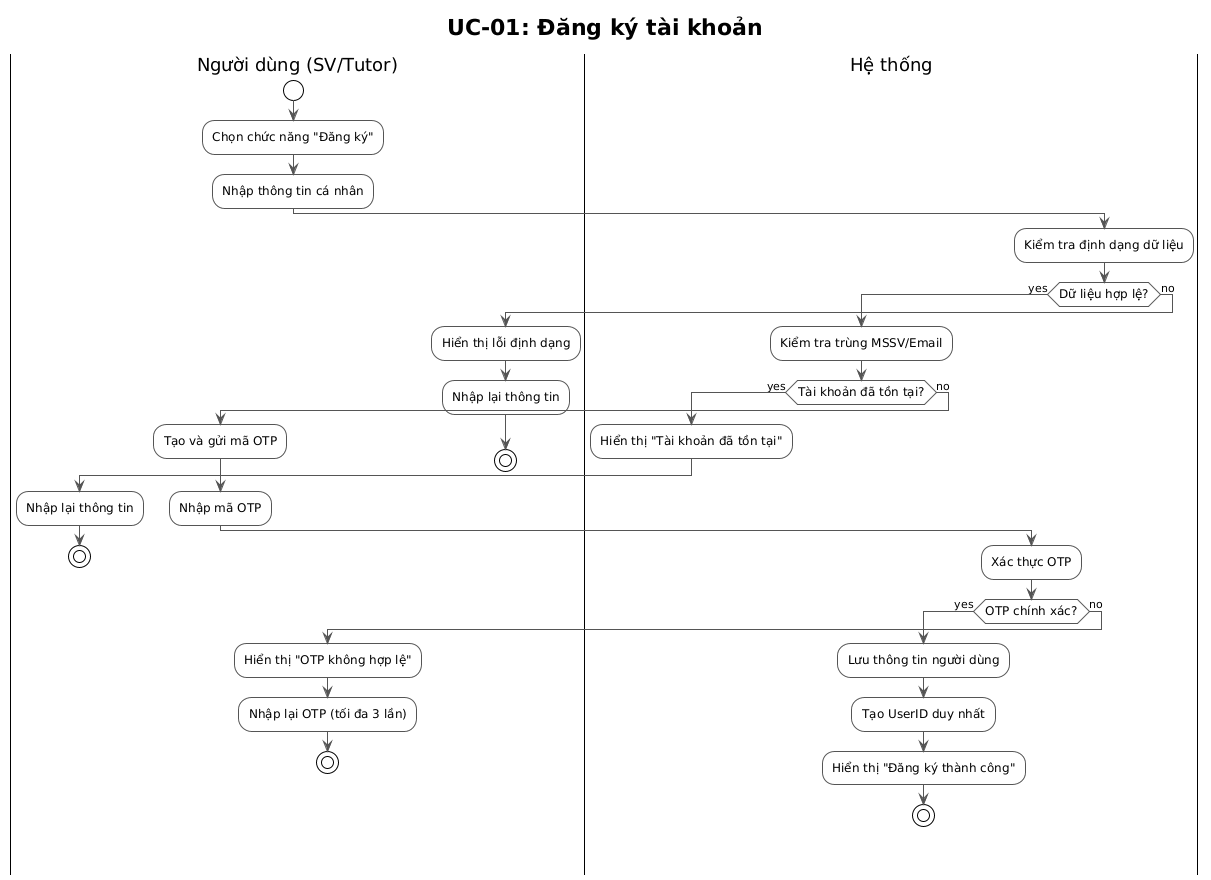
\includegraphics[scale=0.35 ]{Picture/ACUC01.png}
    \caption{Sơ đồ hoạt động Use Case 01: Đăng ký tài khoản}
    \end{figure}
    \item Sơ đồ tuần tự
    \begin{figure}[H]
    \centering
    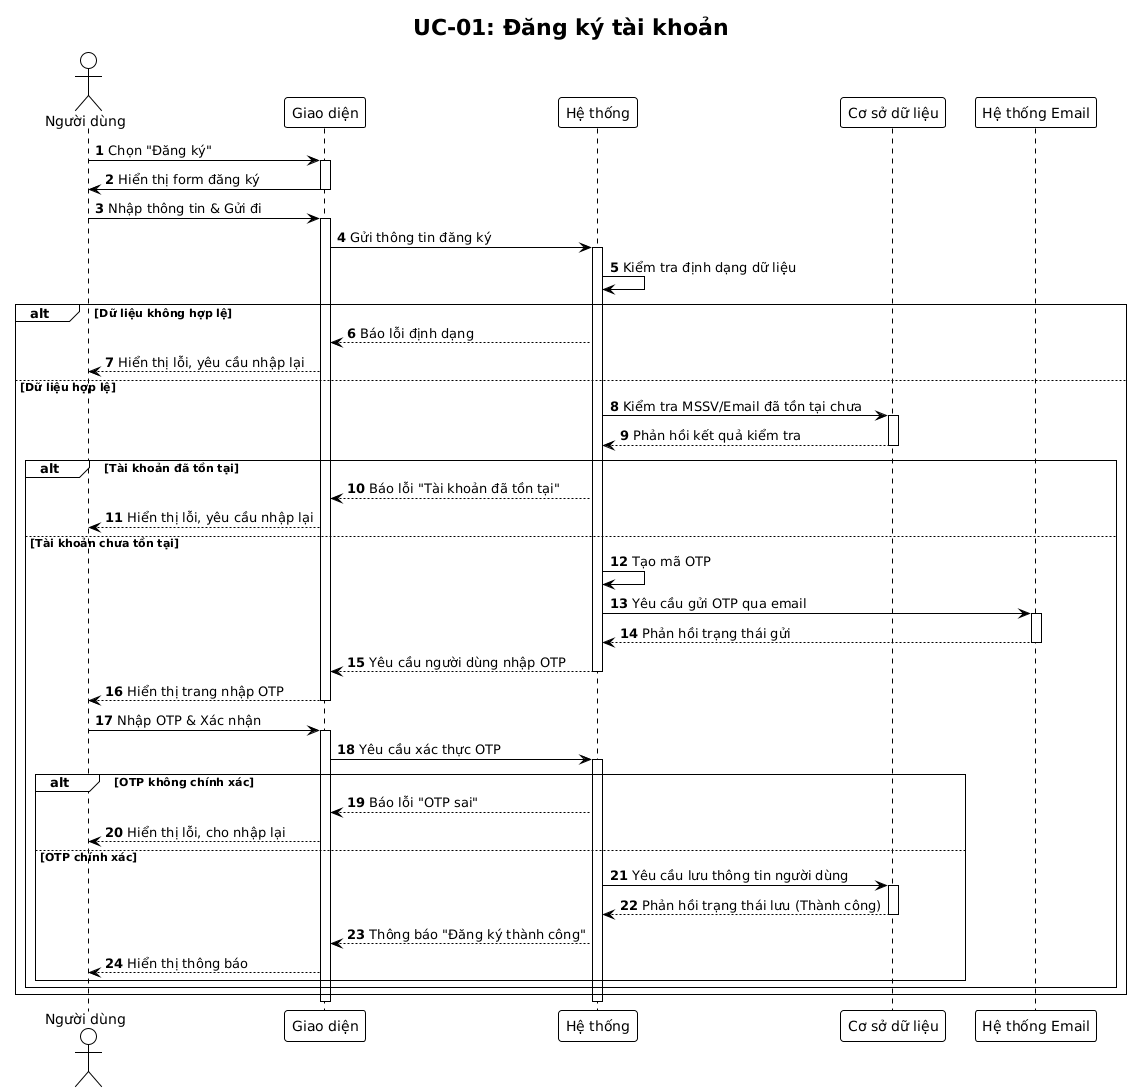
\includegraphics[scale=0.35 ]{Picture/SEUC01.png}
    \caption{Sơ đồ tuần tự Use Case 01: Đăng ký tài khoản}
    \end{figure}
\end{itemize}
%========================================================================================
\subsection*{3.1.2. Use Case 02: Đăng nhập}
\addcontentsline{toc}{subsection}{3.1.2. Use Case 02: Đăng nhập}
\begin{itemize}
    \item Sơ đồ hoạt động
    \begin{figure}[H]
    \centering
    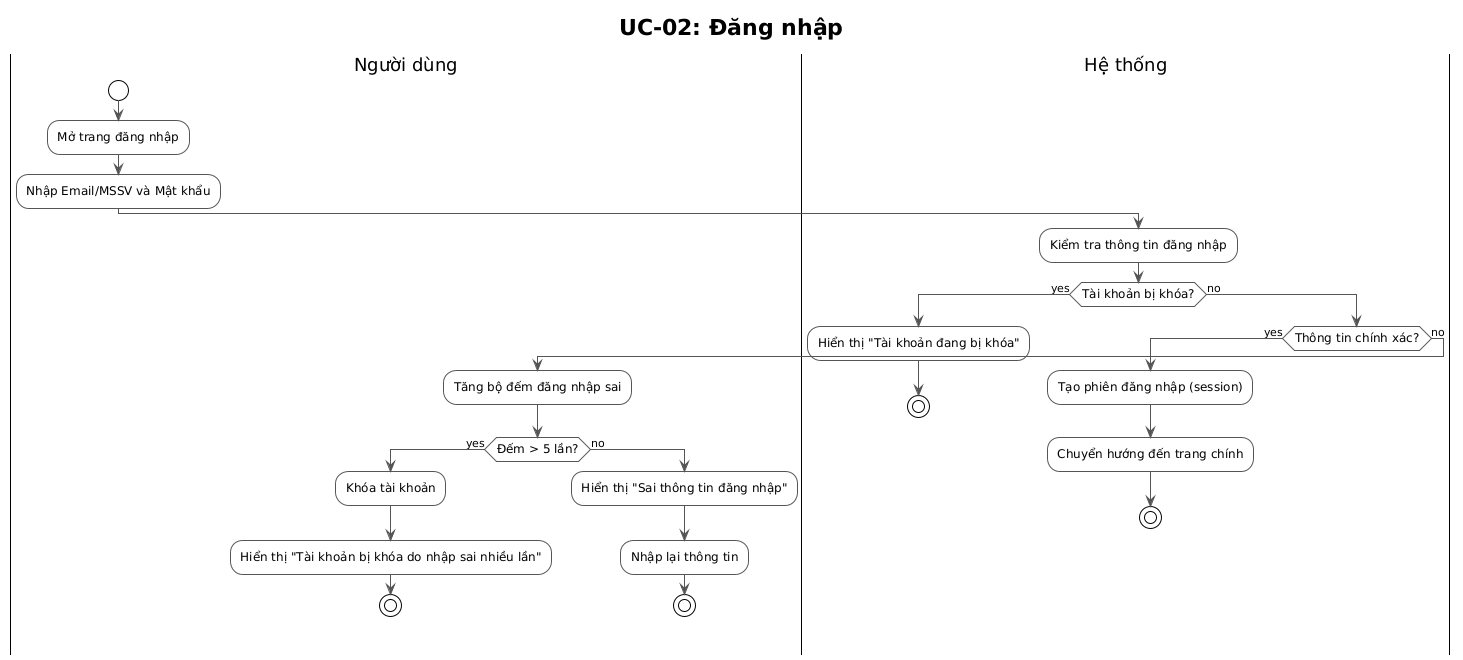
\includegraphics[scale=0.28 ]{Picture/ACUC02.png}
    \caption{Sơ đồ hoạt động Use Case 02: Đăng nhập}
    \end{figure}
    \item Sơ đồ tuần tự
    \begin{figure}[H]
    \centering
    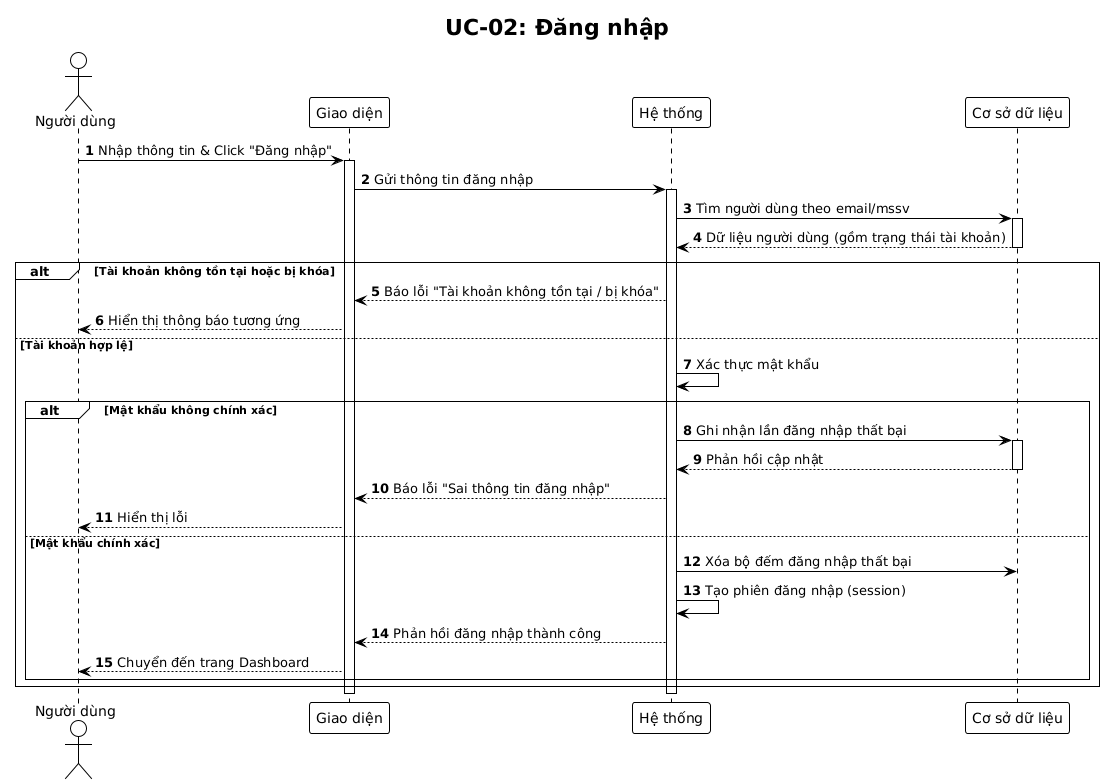
\includegraphics[scale=0.35 ]{Picture/SEUC02.png}
    \caption{Sơ đồ tuần tự Use Case 02: Đăng nhập}
    \end{figure}
\end{itemize}
%========================================================================================
\subsection*{3.1.3. Use Case 03: Cập nhật hồ sơ}
\addcontentsline{toc}{subsection}{3.1.3. Use Case 03: Cập nhật hồ sơ}
\begin{itemize}
    \item Sơ đồ hoạt động
    \begin{figure}[H]
    \centering
    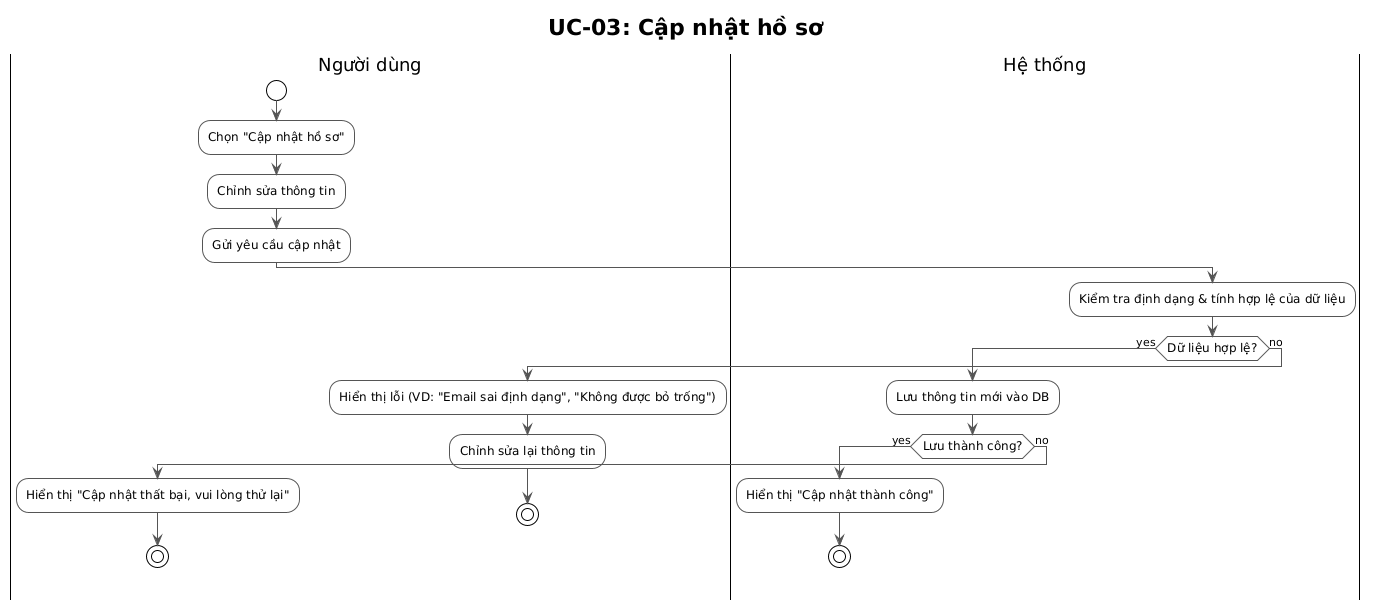
\includegraphics[scale=0.32 ]{Picture/ACUC03.png}
    \caption{Sơ đồ hoạt động Use Case 03: Cập nhật hồ sơ}
    \end{figure}
    \item Sơ đồ tuần tự
    \begin{figure}[H]
    \centering
    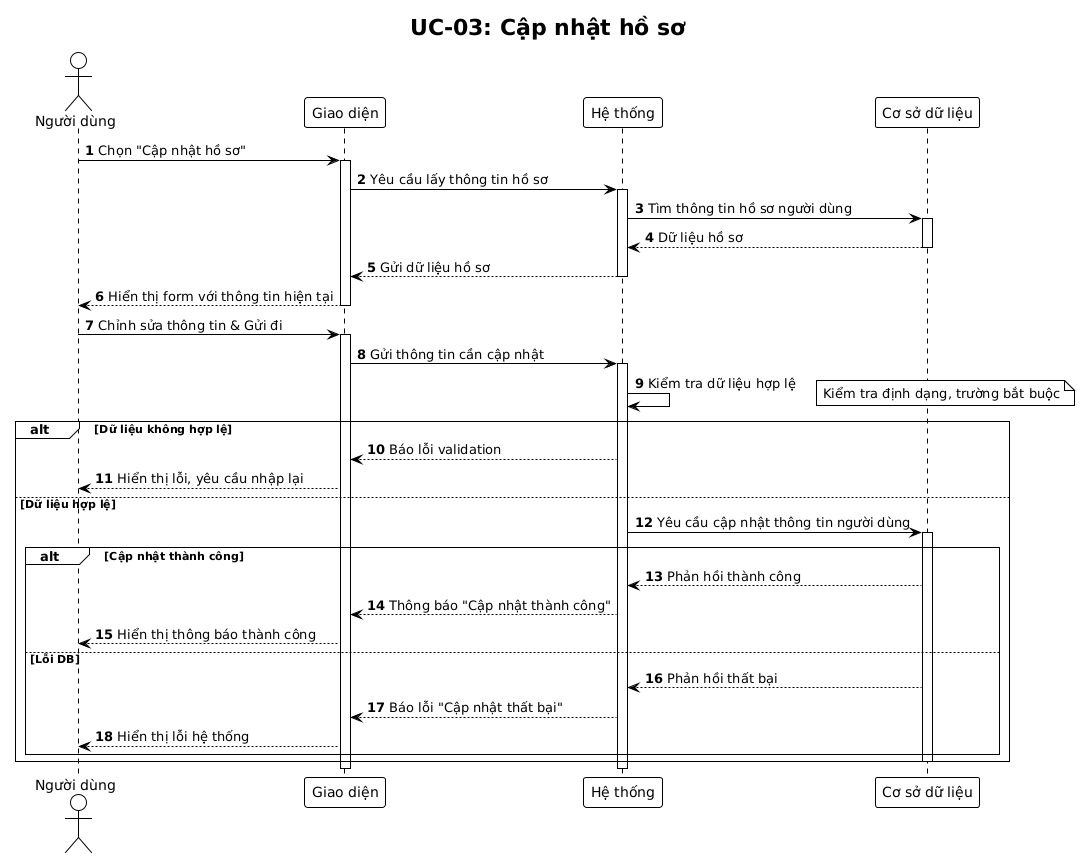
\includegraphics[scale=0.35 ]{Picture/SEUC03.png}
    \caption{Sơ đồ tuần tự Use Case 03: Cập nhật hồ sơ}
    \end{figure}
\end{itemize}
%========================================================================================
\subsection*{3.1.4. Use Case 04: Đăng ký môn học}
\addcontentsline{toc}{subsection}{3.1.4. Use Case 04: Đăng ký môn học}
\begin{itemize}
    \item Sơ đồ hoạt động
    \begin{figure}[H]
    \centering
    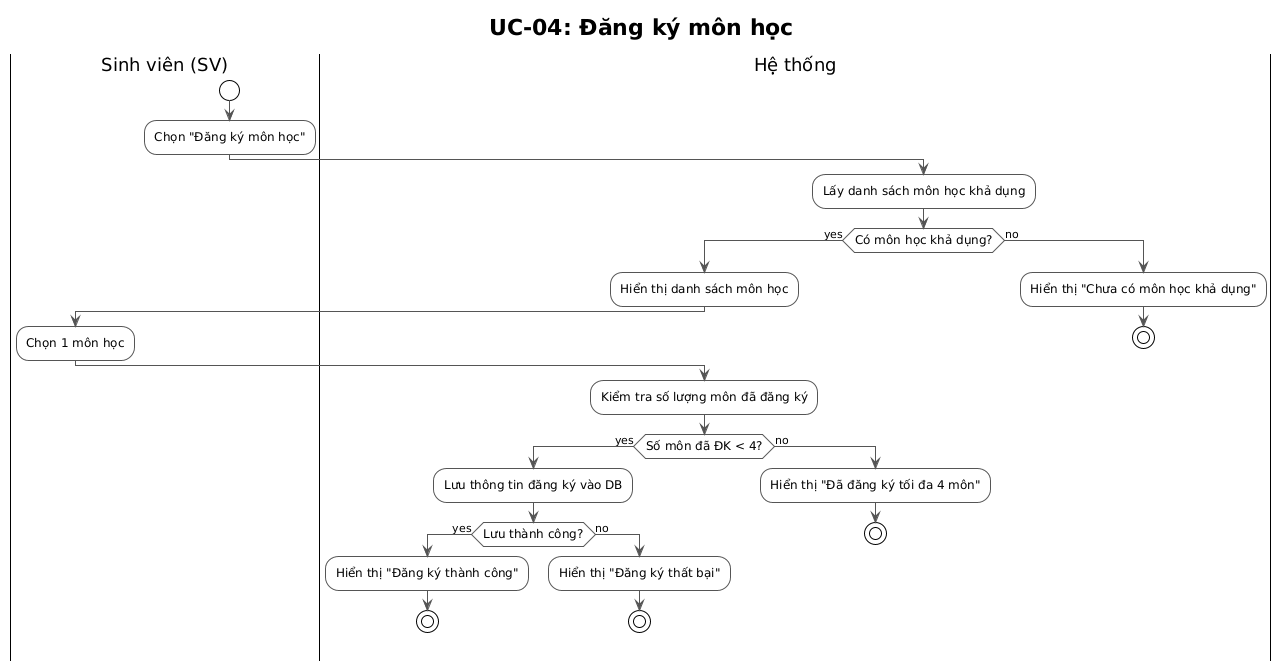
\includegraphics[scale=0.35 ]{Picture/ACUC04.png}
    \caption{Sơ đồ hoạt động Use Case 04: Đăng ký môn học}
    \end{figure}
    \item Sơ đồ tuần tự
    \begin{figure}[H]
    \centering
    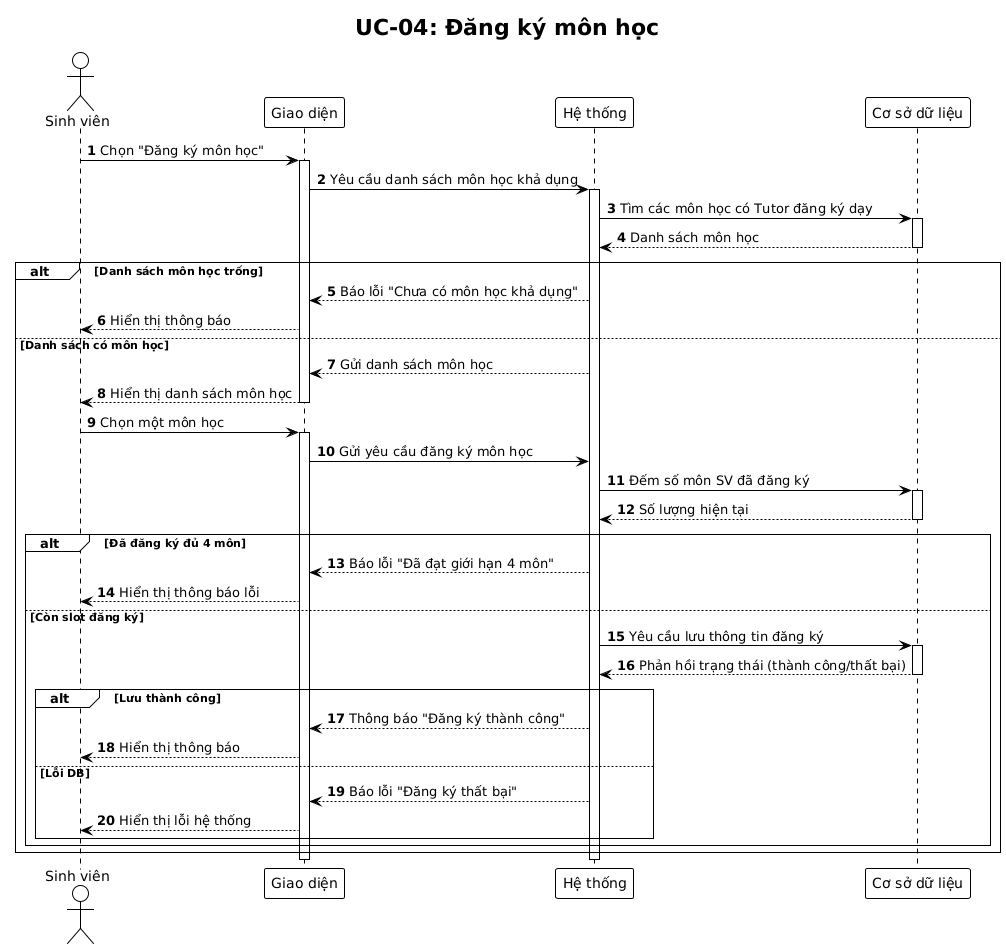
\includegraphics[scale=0.35 ]{Picture/SEUC04.png}
    \caption{Sơ đồ tuần tự Use Case 04: Đăng ký môn học}
    \end{figure}
\end{itemize}
%========================================================================================
\subsection*{3.1.5. Use Case 05: Hủy đăng ký môn học}
\addcontentsline{toc}{subsection}{3.1.5. Use Case 05: Hủy đăng ký môn học}
\begin{itemize}
    \item Sơ đồ hoạt động
    \begin{figure}[H]
    \centering
    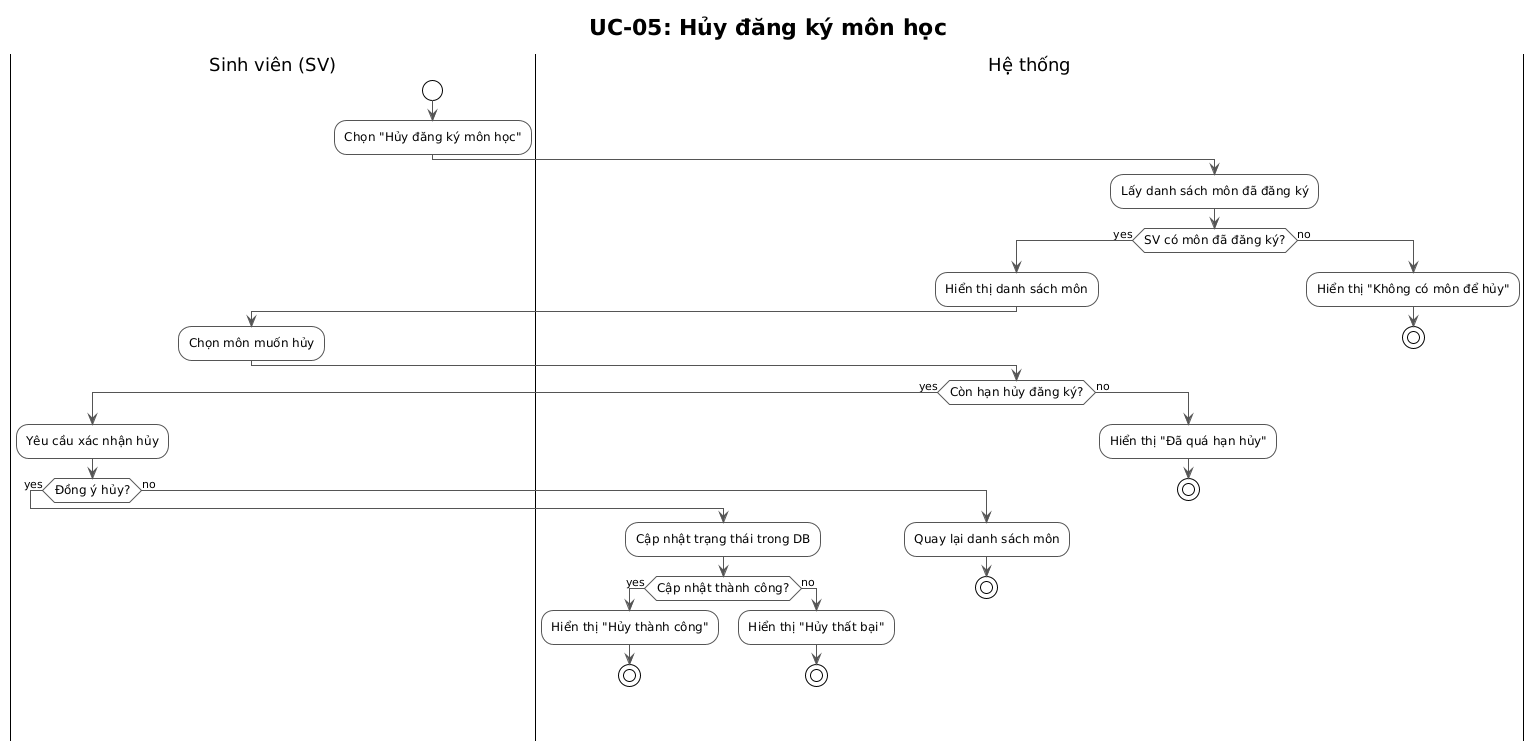
\includegraphics[scale=0.3 ]{Picture/ACUC05.png}
    \caption{Sơ đồ hoạt động Use Case 05: Hủy đăng ký môn học}
    \end{figure}
    \item Sơ đồ tuần tự
    \begin{figure}[H]
    \centering
    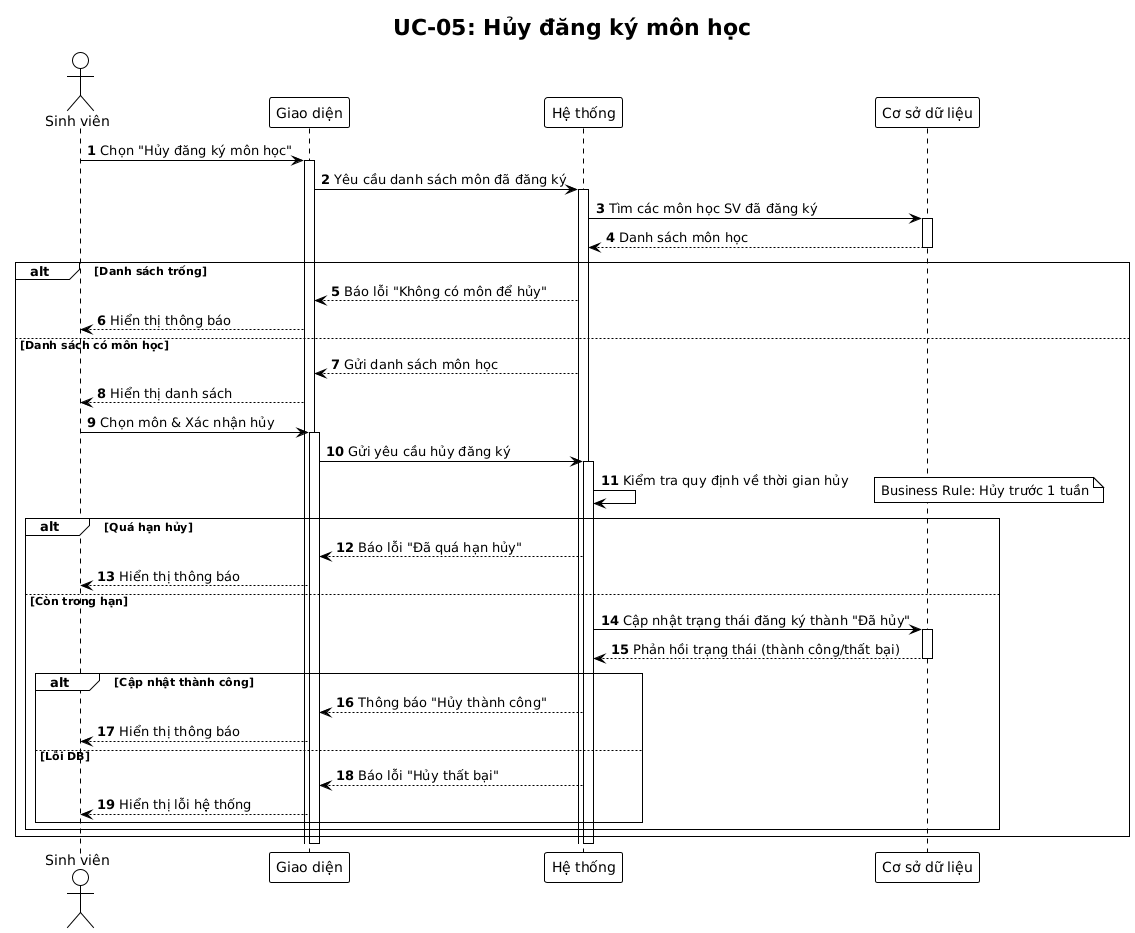
\includegraphics[scale=0.35 ]{Picture/SEUC05.png}
    \caption{Sơ đồ tuần tự Use Case 05: Hủy đăng ký môn học}
    \end{figure}
\end{itemize}
%========================================================================================
\subsection*{3.1.6. Use Case 06: Ghép thủ công (SV chọn Tutor)}
\addcontentsline{toc}{subsection}{3.1.6. Use Case 06: Ghép thủ công (SV chọn Tutor)}
\begin{itemize}
    \item Sơ đồ hoạt động
    \begin{figure}[H]
    \centering
    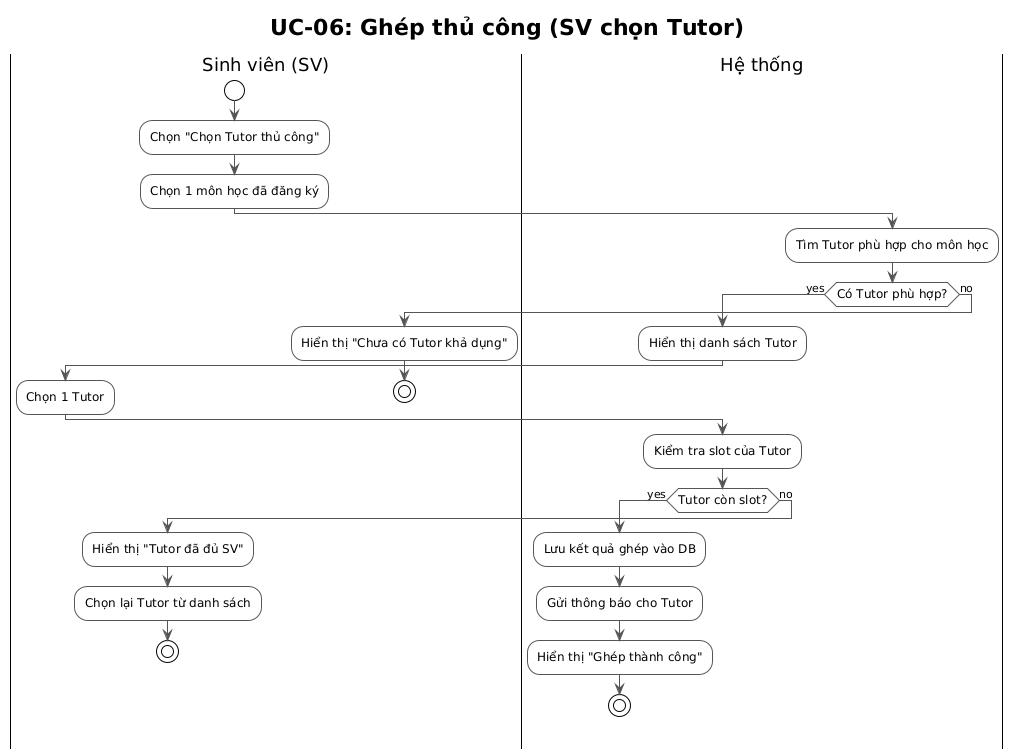
\includegraphics[scale=0.35 ]{Picture/ACUC06.png}
    \caption{Sơ đồ hoạt động Use Case 06: Ghép thủ công (SV chọn Tutor)}
    \end{figure}
    \item Sơ đồ tuần tự
    \begin{figure}[H]
    \centering
    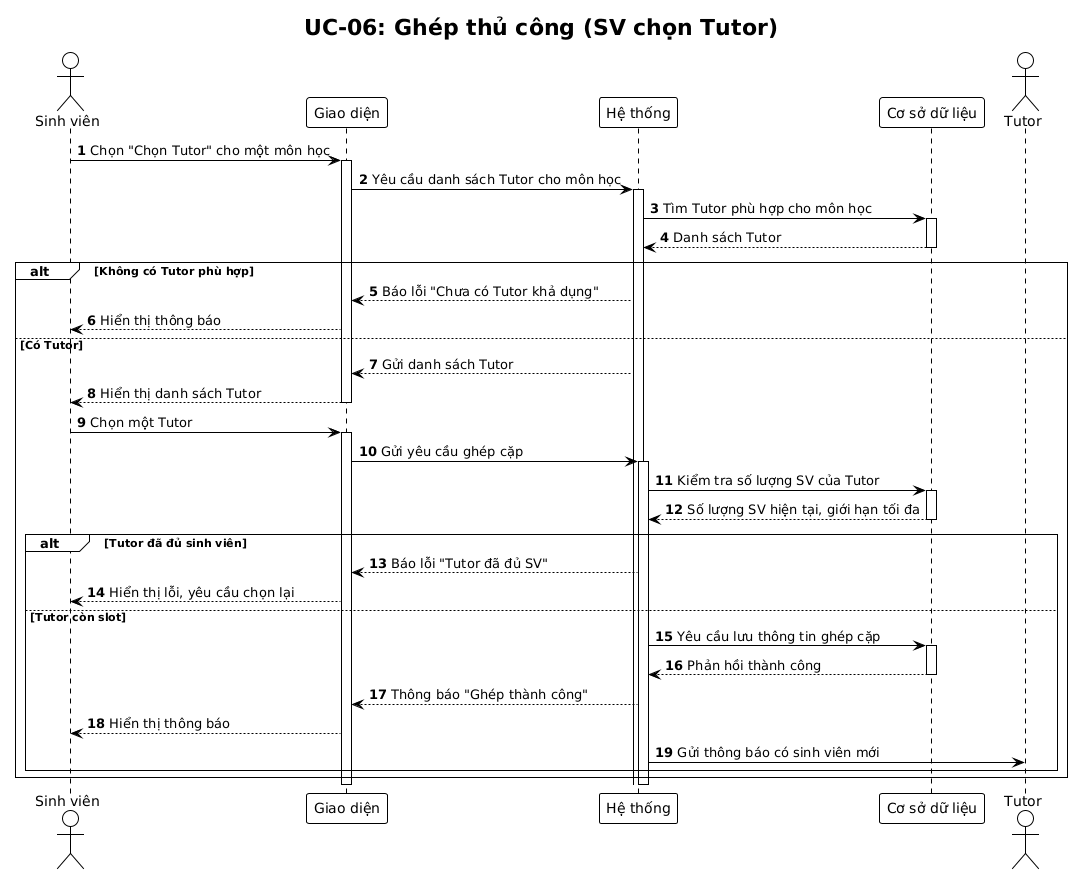
\includegraphics[scale=0.35 ]{Picture/SEUC06.png}
    \caption{Sơ đồ tuần tự Use Case 06: Ghép thủ công (SV chọn Tutor)}
    \end{figure}
\end{itemize}
%========================================================================================
\subsection*{3.1.7. Use Case 07: Ghép tự động (Hệ thống đề xuất Tutor)}
\addcontentsline{toc}{subsection}{3.1.7. Use Case 07: Ghép tự động (Hệ thống đề xuất Tutor)}
\begin{itemize}
    \item Sơ đồ hoạt động
    \begin{figure}[H]
    \centering
    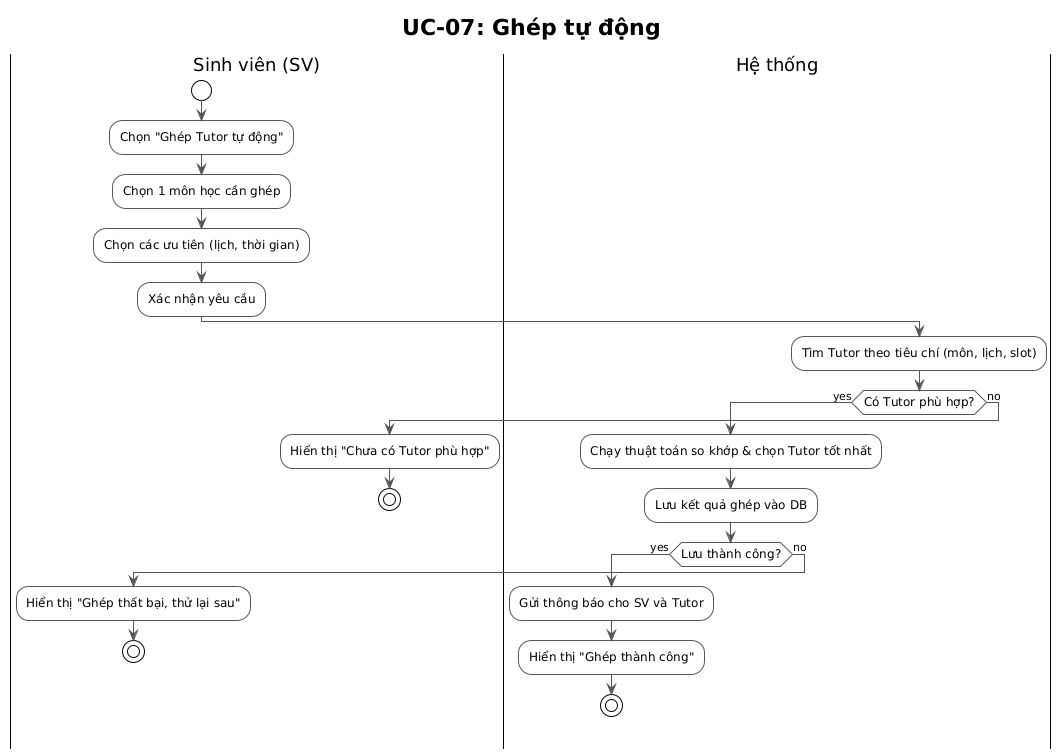
\includegraphics[scale=0.35 ]{Picture/ACUC07.png}
    \caption{Sơ đồ hoạt động Use Case 07: Ghép tự động (Hệ thống đề xuất Tutor)}
    \end{figure}
    \item Sơ đồ tuần tự
    \begin{figure}[H]
    \centering
    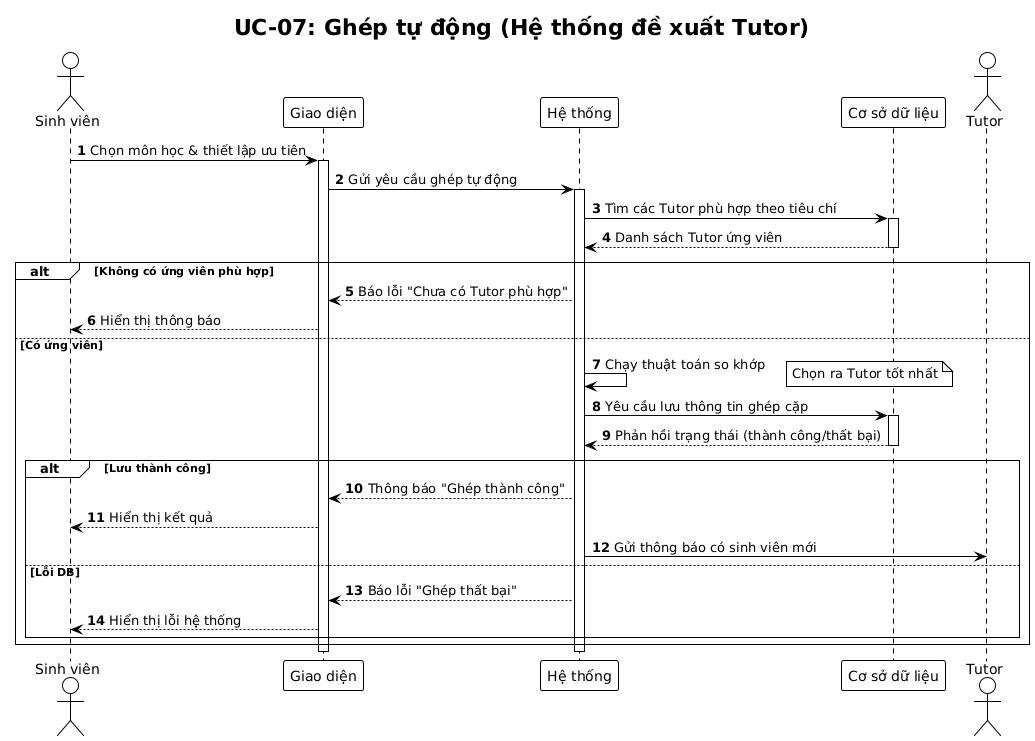
\includegraphics[scale=0.35 ]{Picture/SEUC07.png}
    \caption{Sơ đồ tuần tự Use Case 07: Ghép tự động (Hệ thống đề xuất Tutor)}
    \end{figure}
\end{itemize}
%========================================================================================
\subsection*{3.1.8. Use Case 08: Tạo lịch rảnh (Tutor)}
\addcontentsline{toc}{subsection}{3.1.8. Use Case 08: Tạo lịch rảnh (Tutor)}
\begin{itemize}
    \item Sơ đồ hoạt động
    \begin{figure}[H]
    \centering
    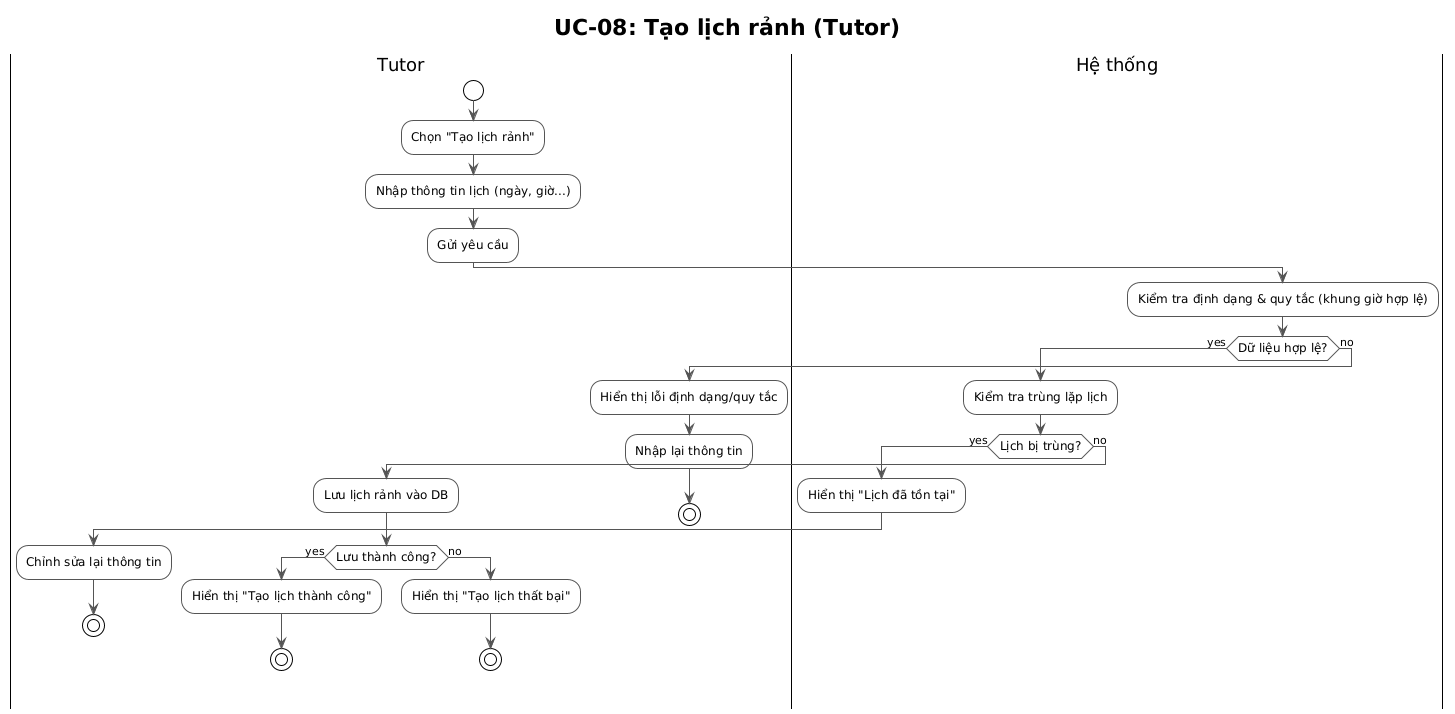
\includegraphics[scale=0.3 ]{Picture/ACUC08.png}
    \caption{Sơ đồ hoạt động Use Case 08: Tạo lịch rảnh (Tutor)}
    \end{figure}
    \item Sơ đồ tuần tự
    \begin{figure}[H]
    \centering
    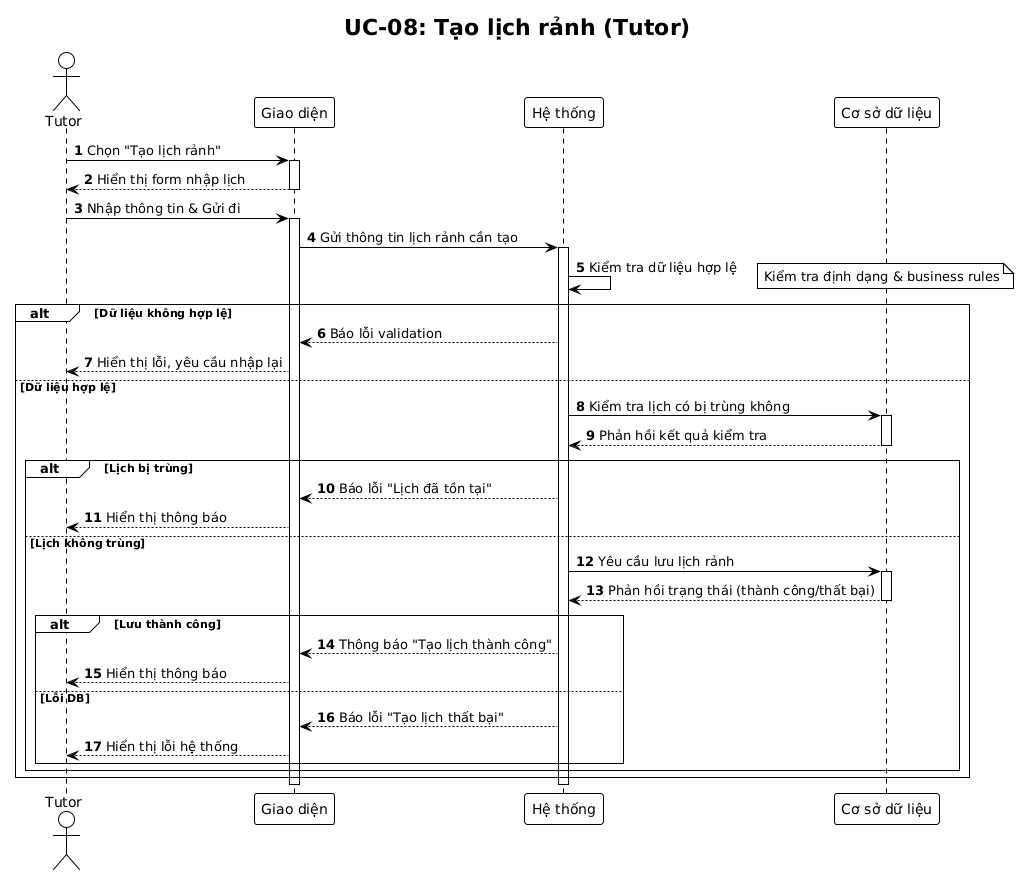
\includegraphics[scale=0.35 ]{Picture/SEUC08.png}
    \caption{Sơ đồ tuần tự Use Case 08: Tạo lịch rảnh (Tutor)}
    \end{figure}
\end{itemize}
%========================================================================================
\subsection*{3.1.9. Use Case 09: Đặt lịch học (SV)}
\addcontentsline{toc}{subsection}{3.1.9. Use Case 09: Đặt lịch học (SV)}
\begin{itemize}
    \item Sơ đồ hoạt động
    \begin{figure}[H]
    \centering
    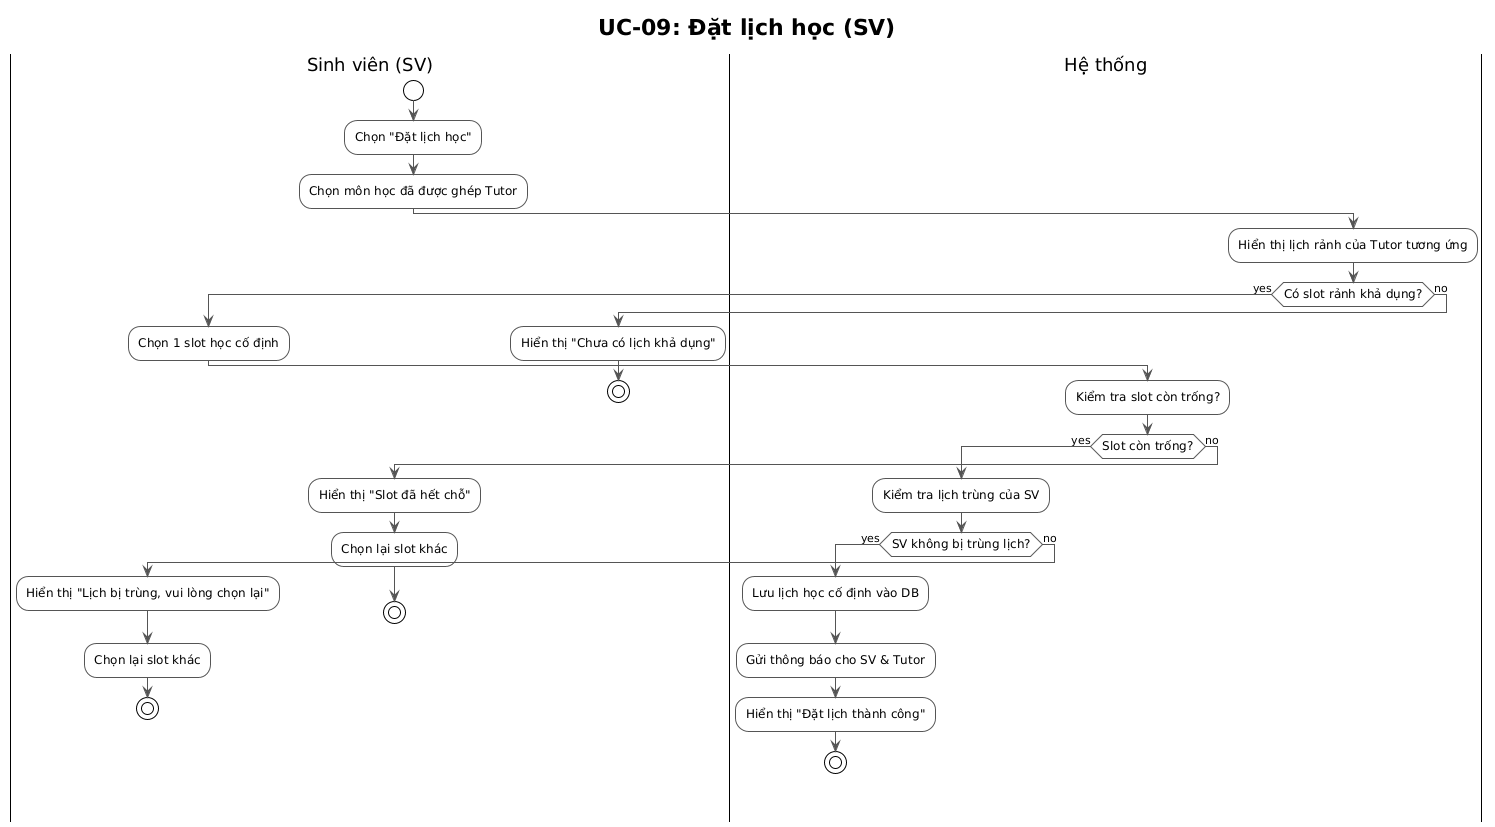
\includegraphics[scale=0.3 ]{Picture/ACUC09.png}
    \caption{Sơ đồ hoạt động Use Case 09: Đặt lịch học (SV)}
    \end{figure}
    \item Sơ đồ tuần tự
    \begin{figure}[H]
    \centering
    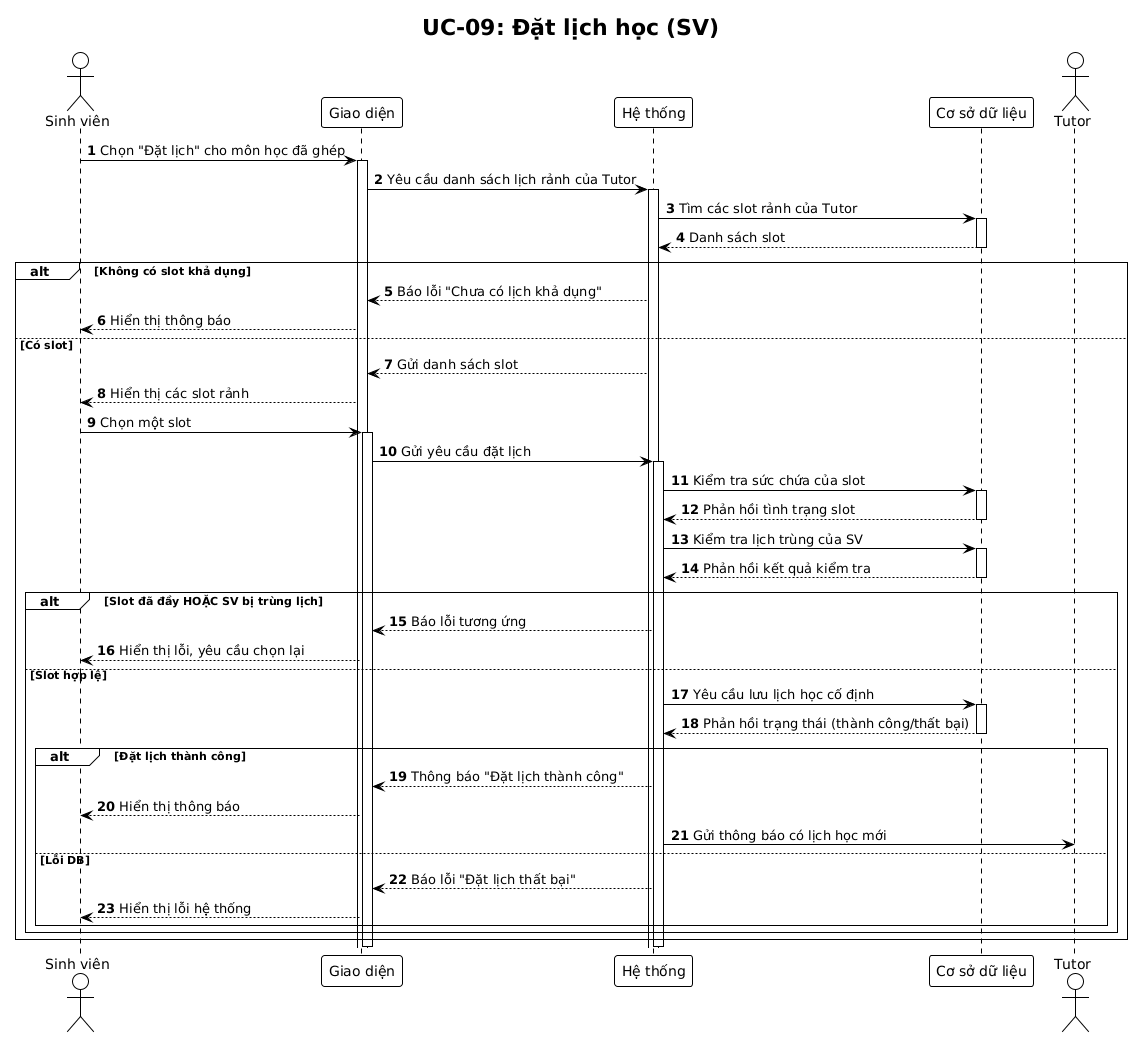
\includegraphics[scale=0.35 ]{Picture/SEUC09.png}
    \caption{Sơ đồ tuần tự Use Case 09: Đặt lịch học (SV)}
    \end{figure}
\end{itemize}
%========================================================================================
\subsection*{3.1.10. Use Case 10: Hủy/Đổi lịch học cố định}
\addcontentsline{toc}{subsection}{3.1.10. Use Case 10: Hủy/Đổi lịch học cố định}
\begin{itemize}
    \item Sơ đồ hoạt động
    \begin{figure}[H]
    \centering
    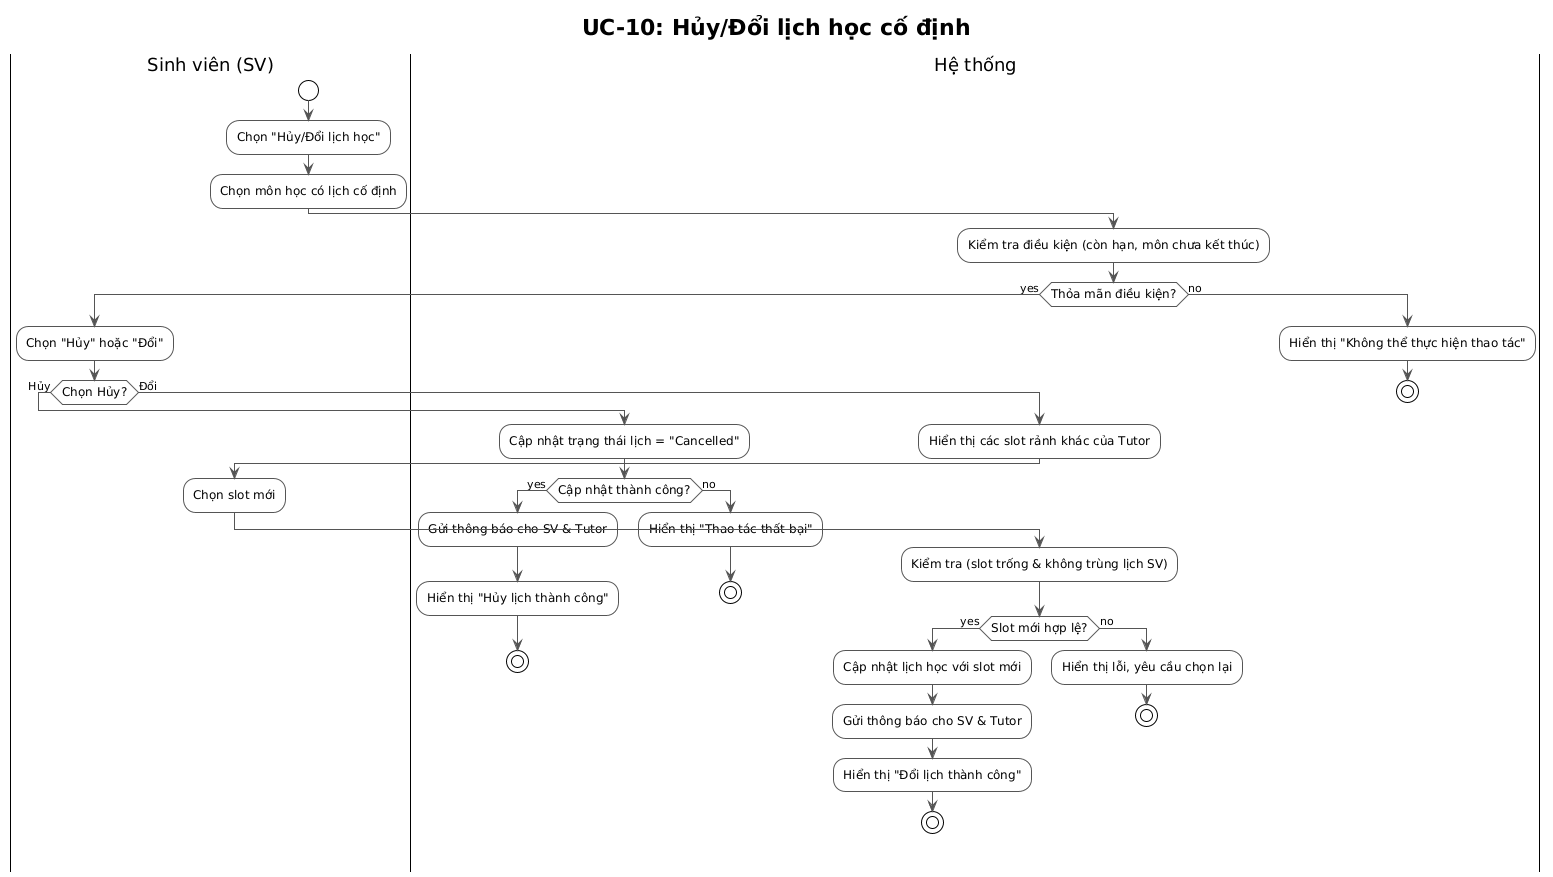
\includegraphics[scale=0.28 ]{Picture/ACUC10.png}
    \caption{Sơ đồ hoạt động Use Case 10: Hủy/Đổi lịch học cố định}
    \end{figure}
    \item Sơ đồ tuần tự
    \begin{figure}[H]
    \centering
    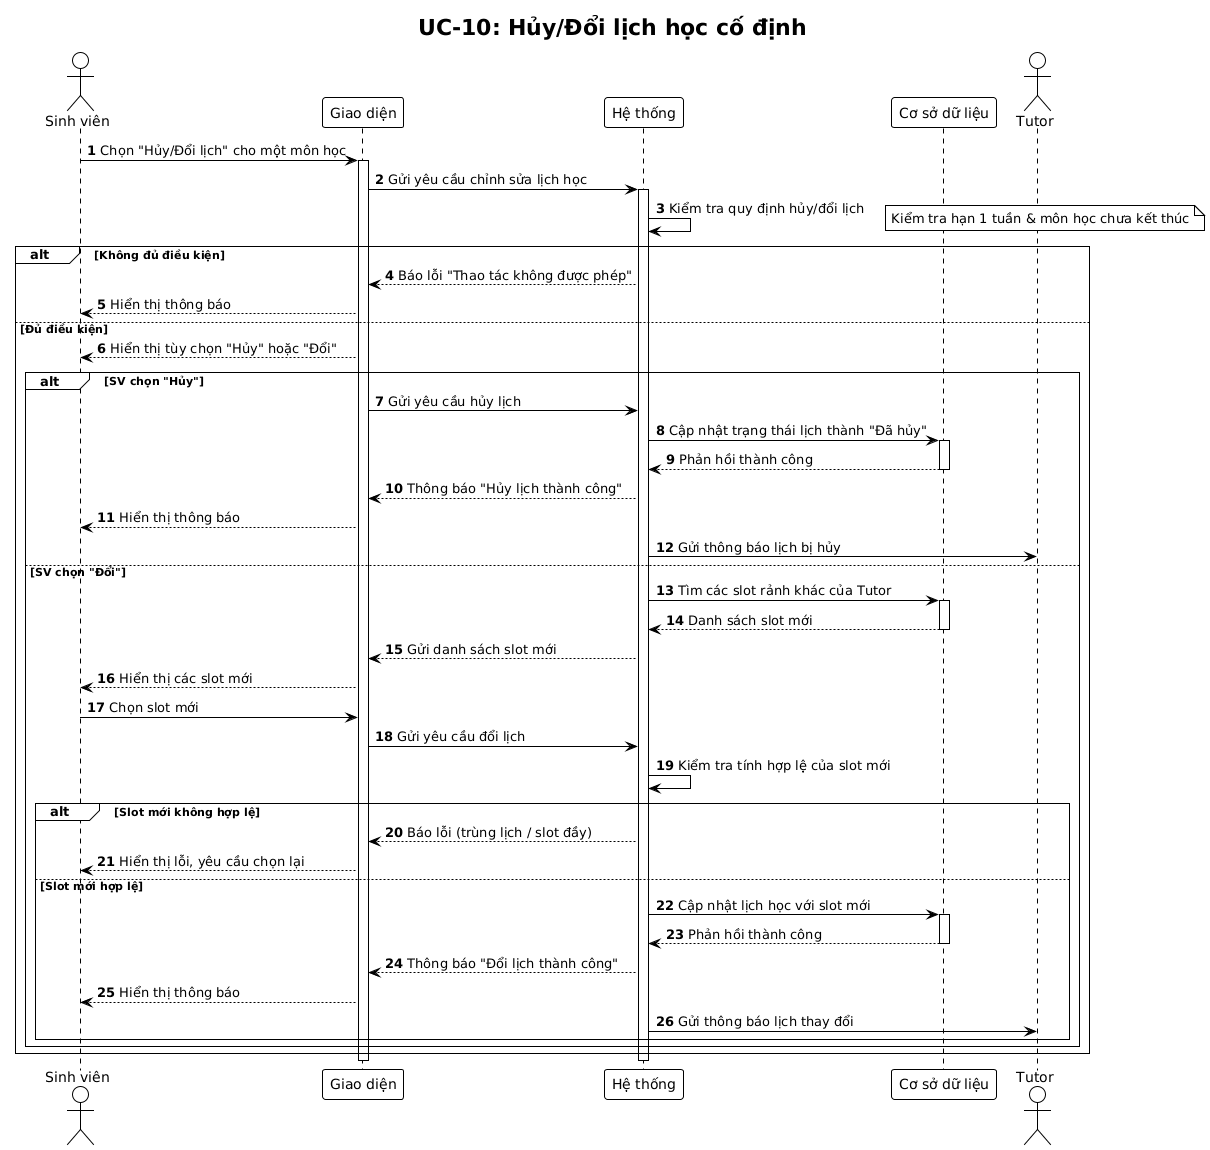
\includegraphics[scale=0.35 ]{Picture/SEUC10.png}
    \caption{Sơ đồ tuần tự Use Case 10: Hủy/Đổi lịch học cố định}
    \end{figure}
\end{itemize}
%========================================================================================
\subsection*{3.1.11. Use Case 11: Gửi thông báo lịch học}
\addcontentsline{toc}{subsection}{3.1.11. Use Case 11: Gửi thông báo lịch học}
\begin{itemize}
    \item Sơ đồ hoạt động
    \begin{figure}[H]
    \centering
    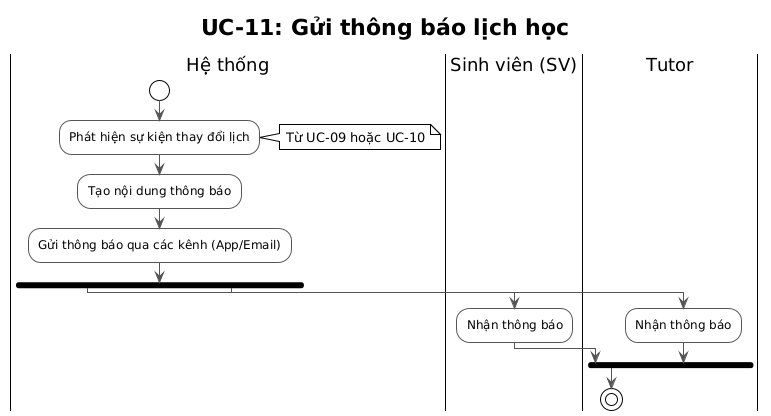
\includegraphics[scale=0.5 ]{Picture/ACUC11.png}
    \caption{Sơ đồ hoạt động Use Case 11: Gửi thông báo lịch học}
    \end{figure}
    \item Sơ đồ tuần tự
    \begin{figure}[H]
    \centering
    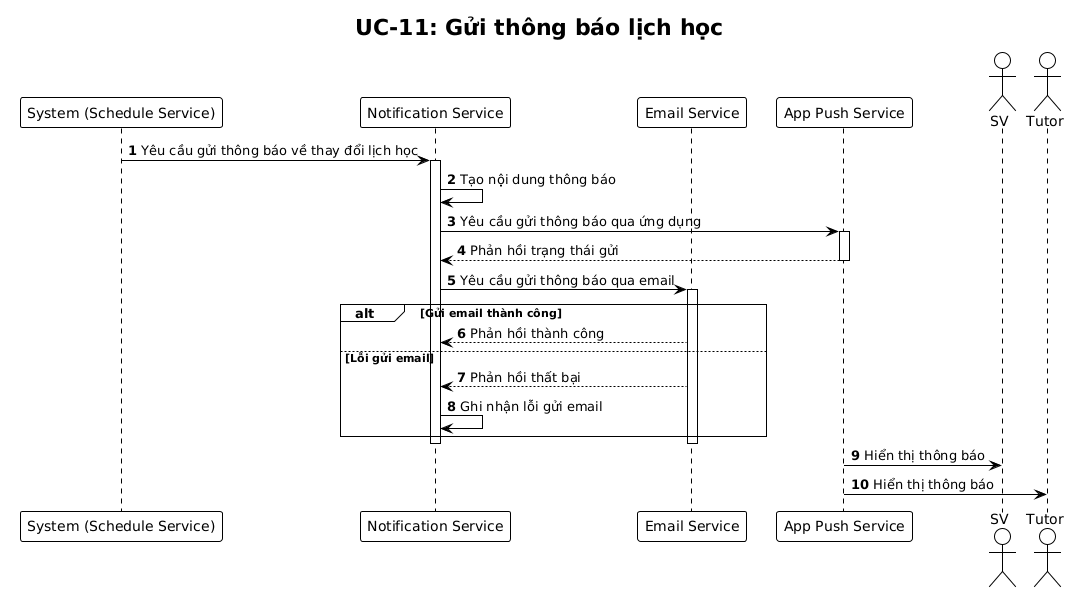
\includegraphics[scale=0.4 ]{Picture/SEUC11.png}
    \caption{Sơ đồ tuần tự Use Case 11: Gửi thông báo lịch học}
    \end{figure}
\end{itemize}
%========================================================================================
\subsection*{3.1.12. Use Case 12: Gửi nhắc nhở buổi học}
\addcontentsline{toc}{subsection}{3.1.12. Use Case 12: Gửi nhắc nhở buổi học}
\begin{itemize}
    \item Sơ đồ hoạt động
    \begin{figure}[H]
    \centering
    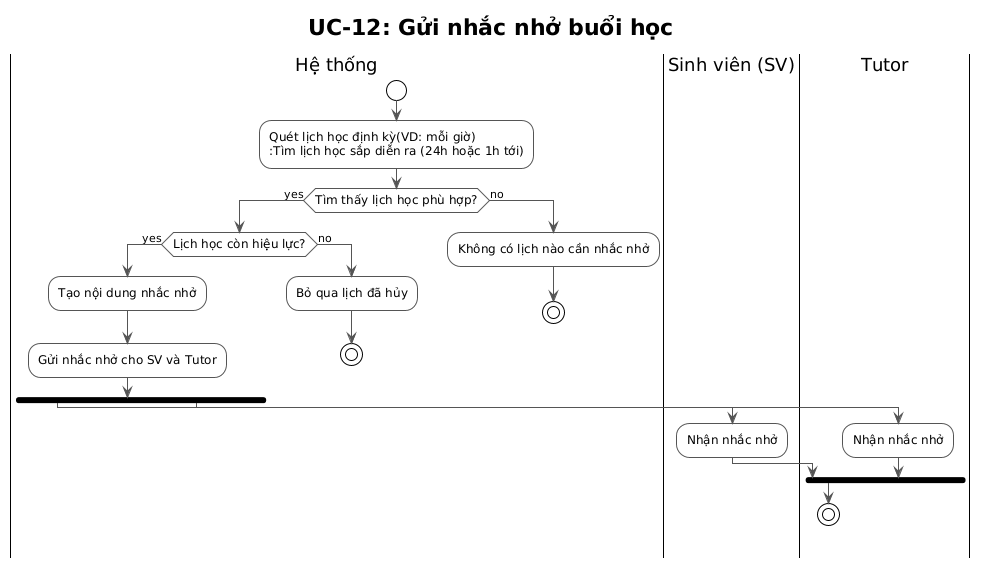
\includegraphics[scale=0.4 ]{Picture/ACUC12.png}
    \caption{Sơ đồ hoạt động Use Case 12: Gửi nhắc nhở buổi học}
    \end{figure}
    \item Sơ đồ tuần tự
    \begin{figure}[H]
    \centering
    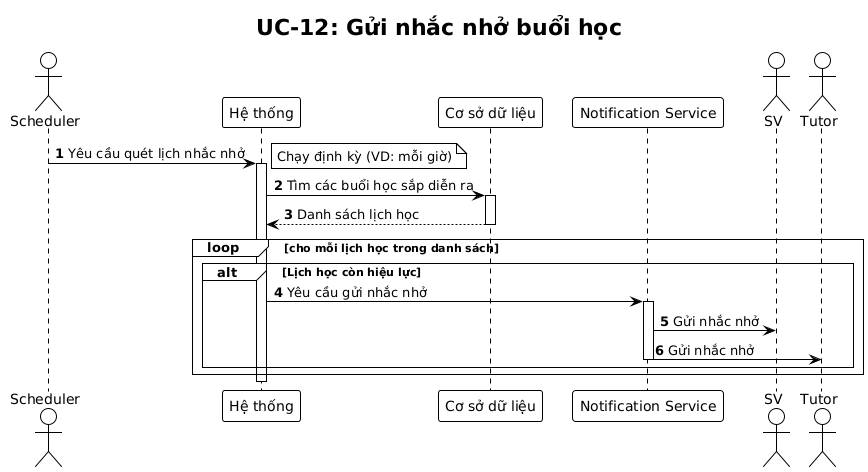
\includegraphics[scale=0.4 ]{Picture/SEUC12.png}
    \caption{Sơ đồ tuần tự Use Case 12: Gửi nhắc nhở buổi học}
    \end{figure}
\end{itemize}
%========================================================================================
\subsection*{3.1.13. Use Case 13: Điểm danh sinh viên}
\addcontentsline{toc}{subsection}{3.1.13. Use Case 13: Điểm danh sinh viên}
\begin{itemize}
    \item Sơ đồ hoạt động
    \begin{figure}[H]
    \centering
    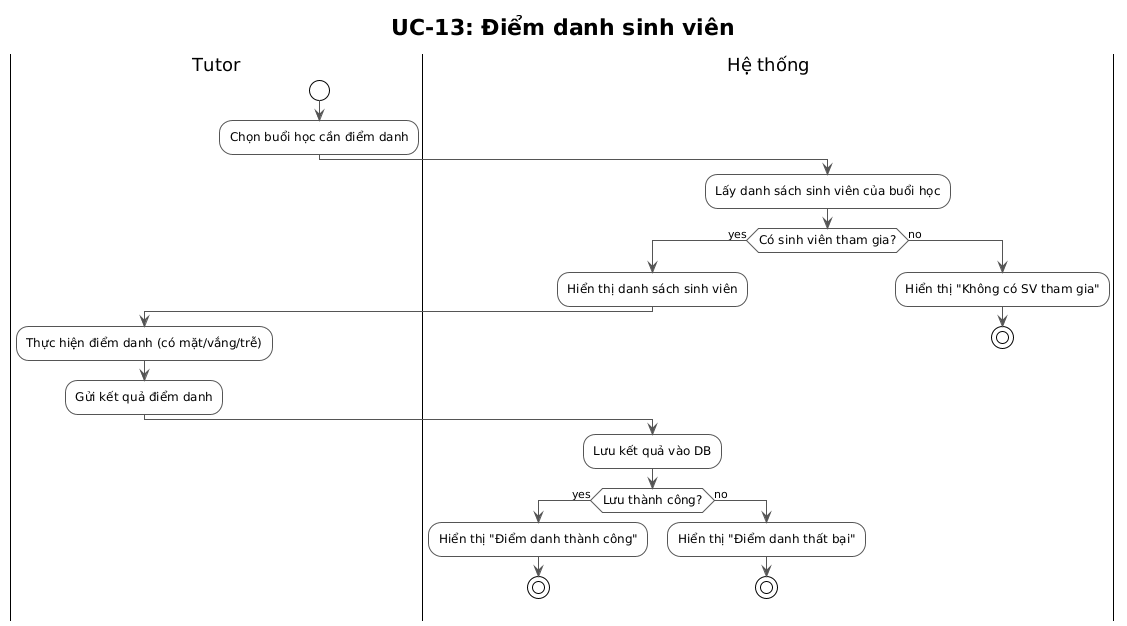
\includegraphics[scale=0.35 ]{Picture/ACUC13.png}
    \caption{Sơ đồ hoạt động Use Case 13: Điểm danh sinh viên}
    \end{figure}
    \item Sơ đồ tuần tự
    \begin{figure}[H]
    \centering
    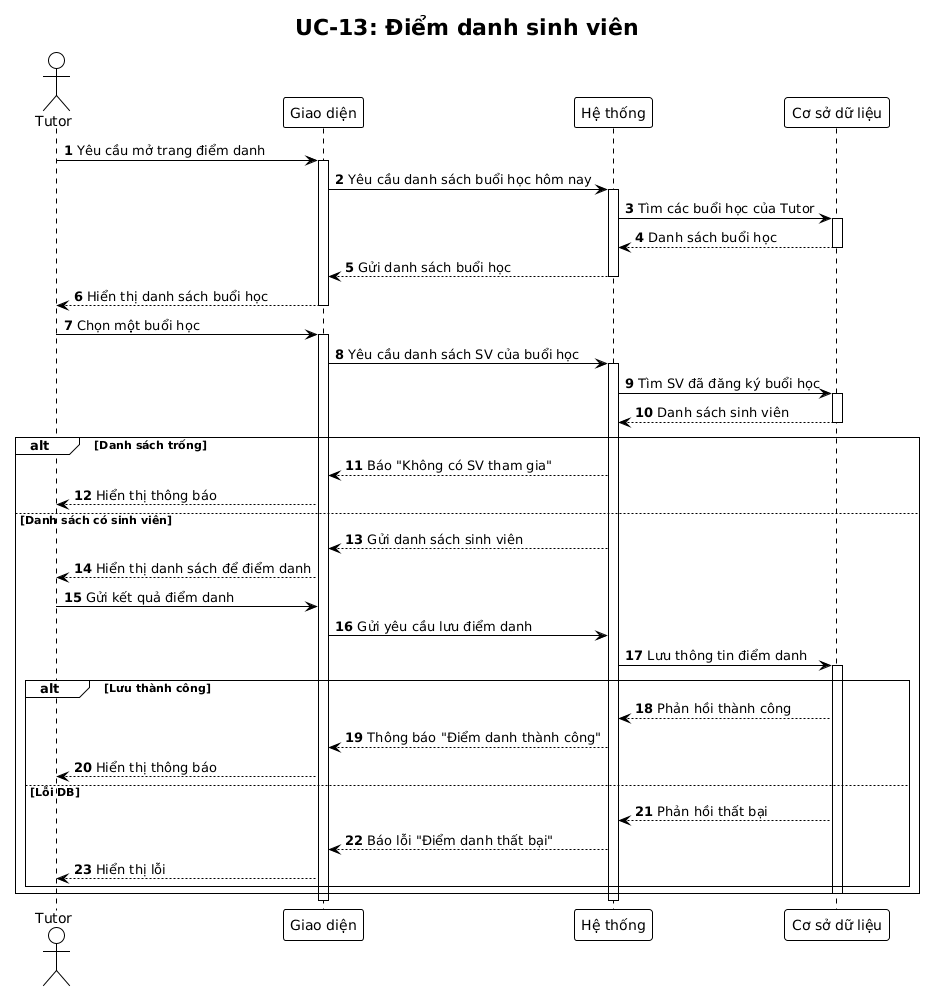
\includegraphics[scale=0.35 ]{Picture/SEUC13.png}
    \caption{Sơ đồ tuần tự Use Case 13: Điểm danh sinh viên}
    \end{figure}
\end{itemize}
%========================================================================================
\subsection*{3.1.14. Use Case 14: Cập nhật trạng thái buổi học}
\addcontentsline{toc}{subsection}{3.1.14. Use Case 14: Cập nhật trạng thái buổi học}
\begin{itemize}
    \item Sơ đồ hoạt động
    \begin{figure}[H]
    \centering
    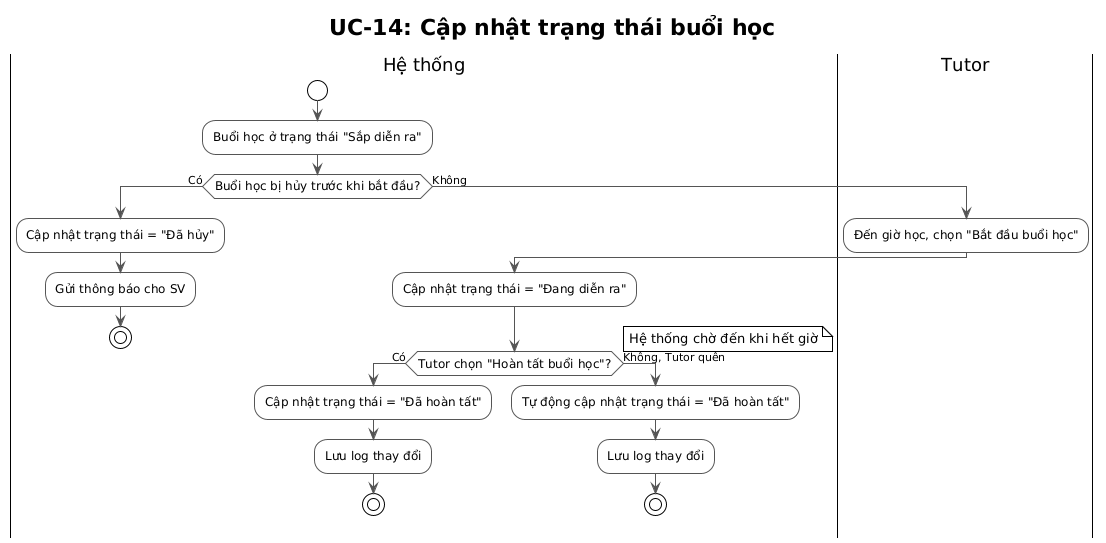
\includegraphics[scale=0.35 ]{Picture/ACUC14.png}
    \caption{Sơ đồ hoạt động Use Case 14: Cập nhật trạng thái buổi học}
    \end{figure}
    \item Sơ đồ tuần tự
    \begin{figure}[H]
    \centering
    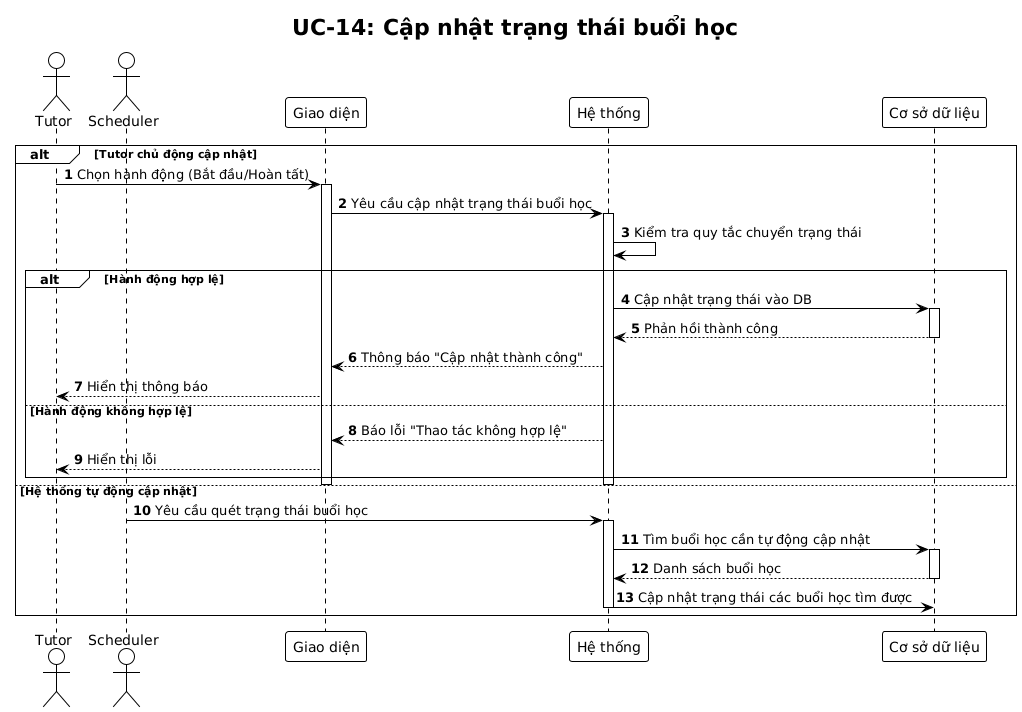
\includegraphics[scale=0.35 ]{Picture/SEUC14.png}
    \caption{Sơ đồ tuần tự Use Case 14: Cập nhật trạng thái buổi học}
    \end{figure}
\end{itemize}
%========================================================================================
\subsection*{3.1.15. Use Case 15: Quản lý tài liệu (Tutor)}
\addcontentsline{toc}{subsection}{3.1.15. Use Case 15: Quản lý tài liệu (Tutor)}
\begin{itemize}
    \item Sơ đồ hoạt động
    \begin{figure}[H]
    \centering
    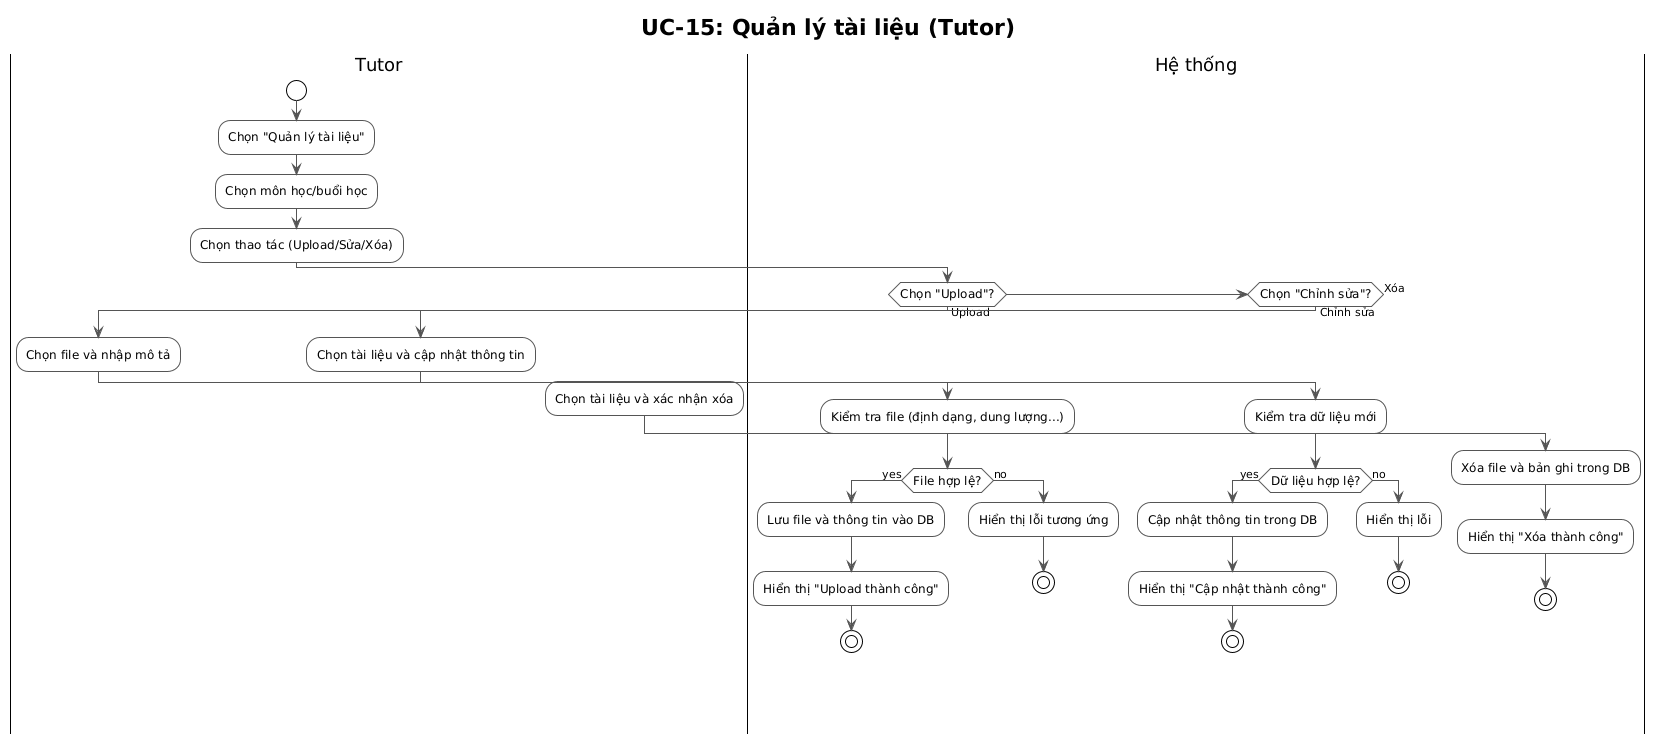
\includegraphics[scale=0.28 ]{Picture/ACUC15.png}
    \caption{Sơ đồ hoạt động Use Case 15: Quản lý tài liệu (Tutor)}
    \end{figure}
    \item Sơ đồ tuần tự
    \begin{figure}[H]
    \centering
    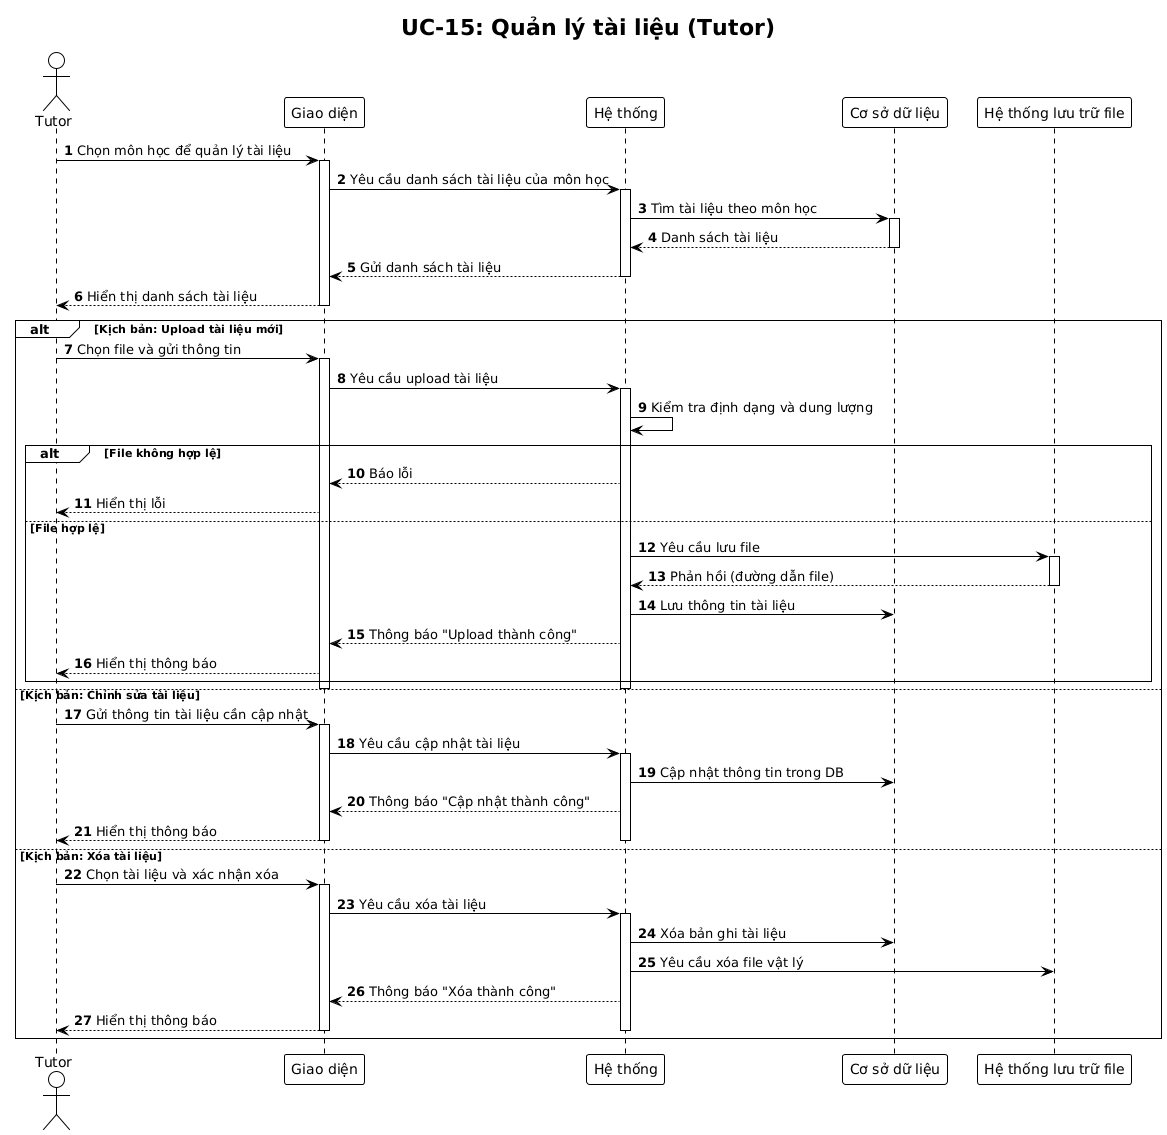
\includegraphics[scale=0.35 ]{Picture/SEUC15.png}
    \caption{Sơ đồ tuần tự Use Case 15: Quản lý tài liệu (Tutor)}
    \end{figure}
\end{itemize}
%========================================================================================
\subsection*{3.1.16. Use Case 16: SV tải tài liệu}
\addcontentsline{toc}{subsection}{3.1.16. Use Case 16: SV tải tài liệu}
\begin{itemize}
    \item Sơ đồ hoạt động
    \begin{figure}[H]
    \centering
    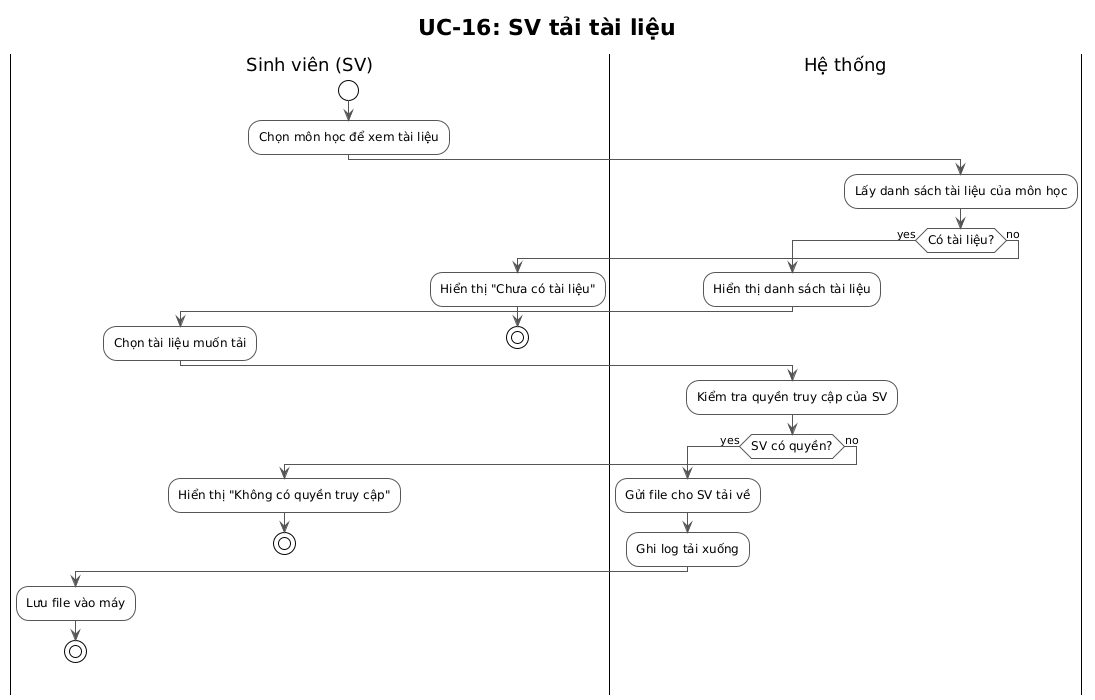
\includegraphics[scale=0.35 ]{Picture/ACUC16.png}
    \caption{Sơ đồ hoạt động Use Case 16: SV tải tài liệu}
    \end{figure}
    \item Sơ đồ tuần tự
    \begin{figure}[H]
    \centering
    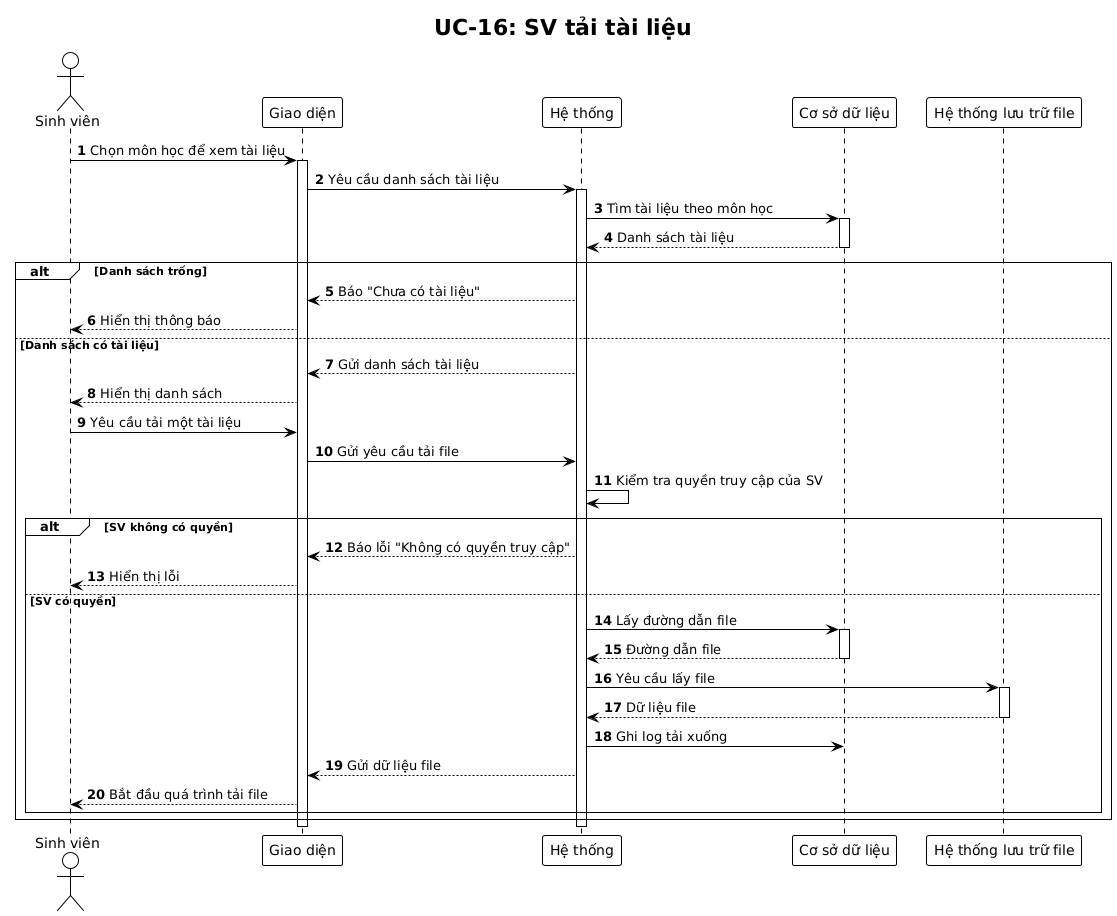
\includegraphics[scale=0.35 ]{Picture/SEUC16.png}
    \caption{Sơ đồ tuần tự Use Case 16: SV tải tài liệu}
    \end{figure}
\end{itemize}
%========================================================================================
\subsection*{3.1.17. Use Case 17: SV đánh giá Tutor}
\addcontentsline{toc}{subsection}{3.1.17. Use Case 17: SV đánh giá Tutor}
\begin{itemize}
    \item Sơ đồ hoạt động
    \begin{figure}[H]
    \centering
    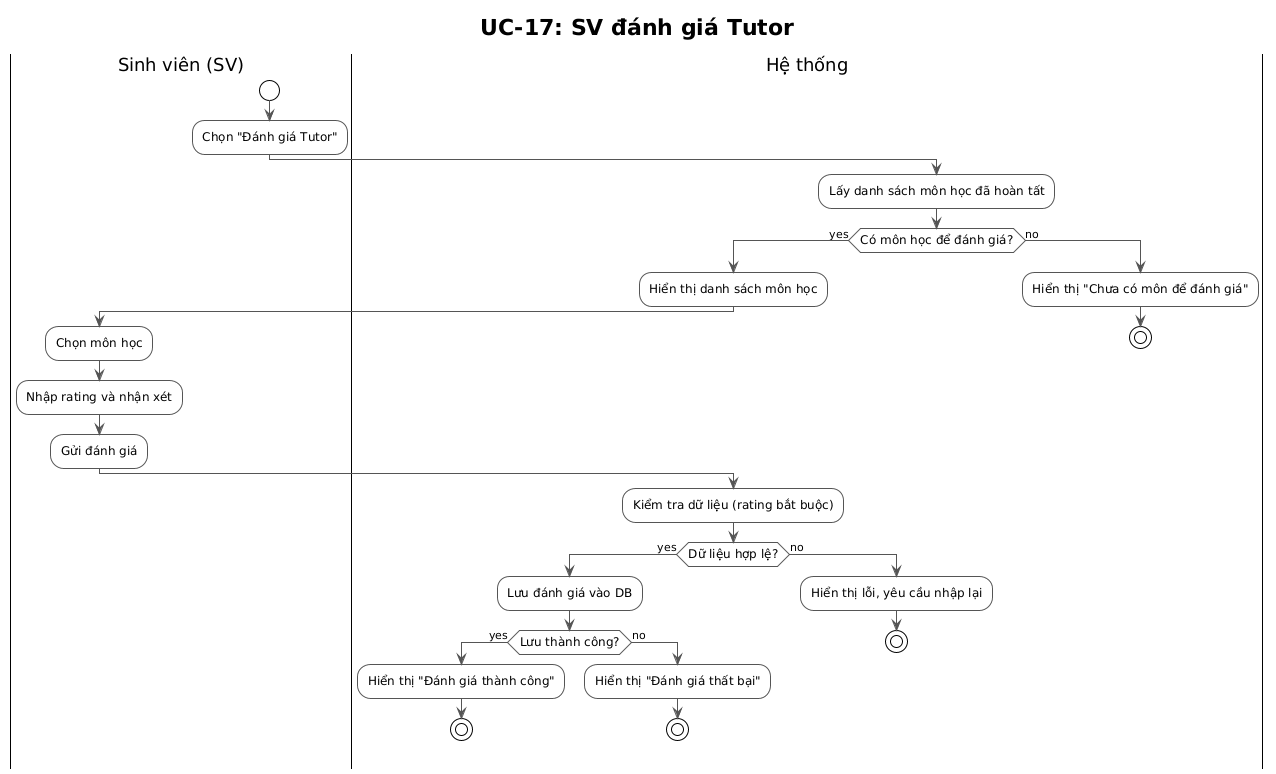
\includegraphics[scale=0.35 ]{Picture/ACUC17.png}
    \caption{Sơ đồ hoạt động Use Case 17: SV đánh giá Tutor}
    \end{figure}
    \item Sơ đồ tuần tự
    \begin{figure}[H]
    \centering
    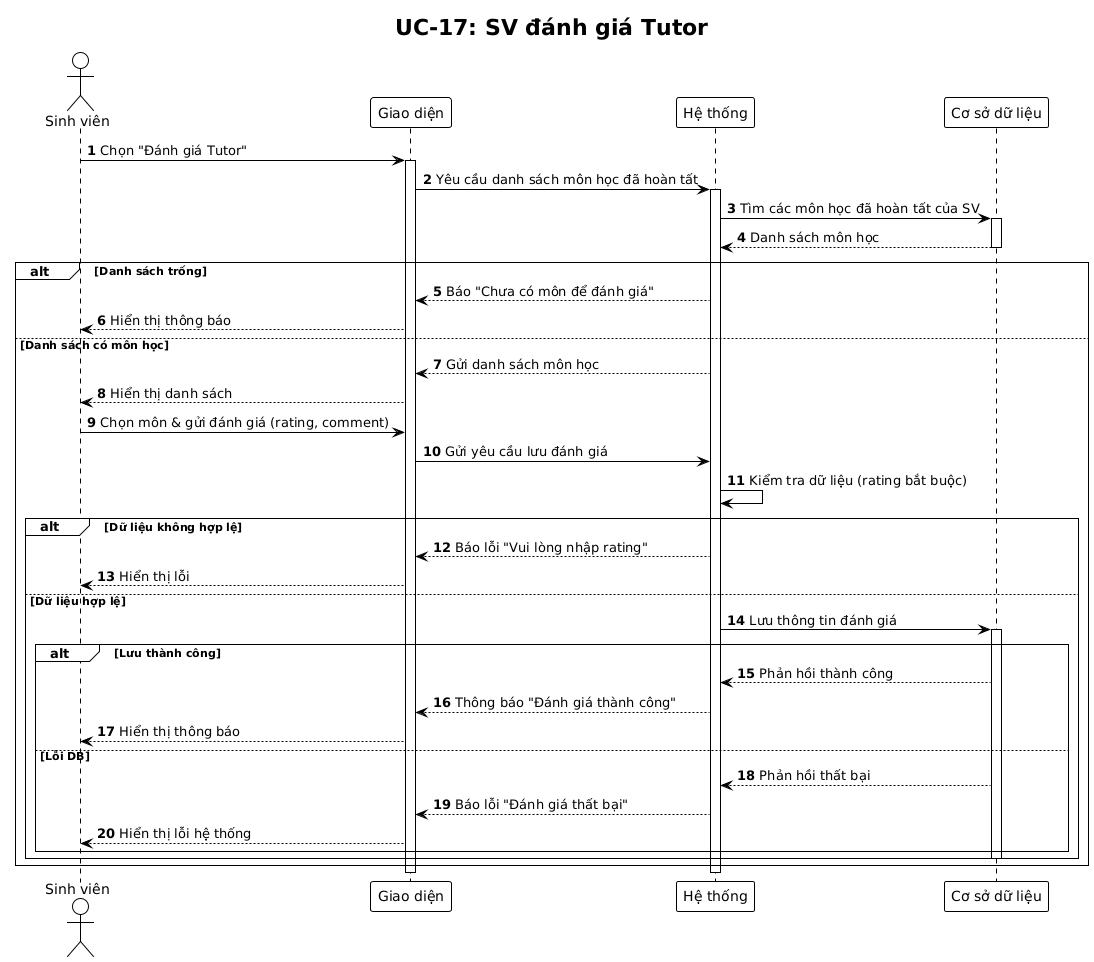
\includegraphics[scale=0.35 ]{Picture/SEUC17.png}
    \caption{Sơ đồ tuần tự Use Case 17: SV đánh giá Tutor}
    \end{figure}
\end{itemize}
%========================================================================================
\subsection*{3.1.18. Use Case 18: Tutor đánh giá sinh viên}
\addcontentsline{toc}{subsection}{3.1.18. Use Case 18: Tutor đánh giá sinh viên}
\begin{itemize}
    \item Sơ đồ hoạt động
    \begin{figure}[H]
    \centering
    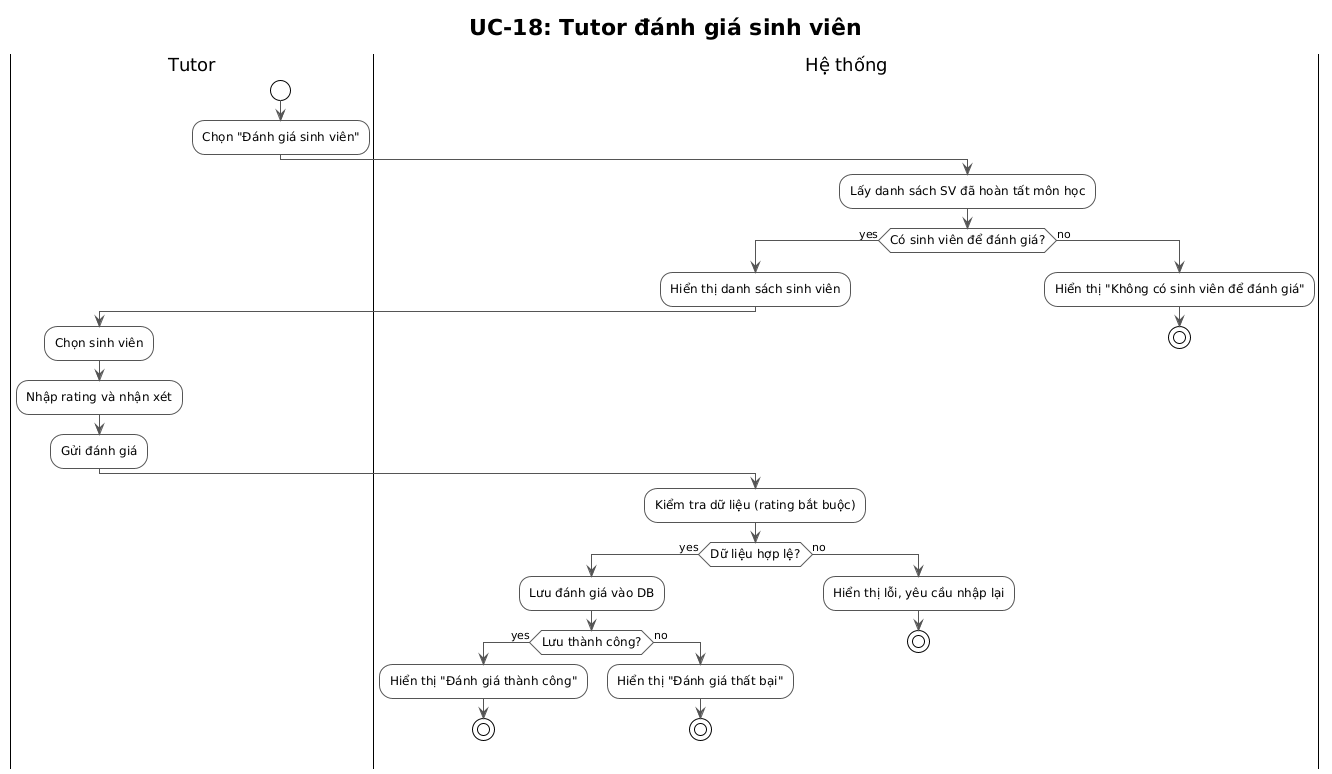
\includegraphics[scale=0.35 ]{Picture/ACUC18.png}
    \caption{Sơ đồ hoạt động Use Case 18: Tutor đánh giá sinh viên}
    \end{figure}
    \item Sơ đồ tuần tự
    \begin{figure}[H]
    \centering
    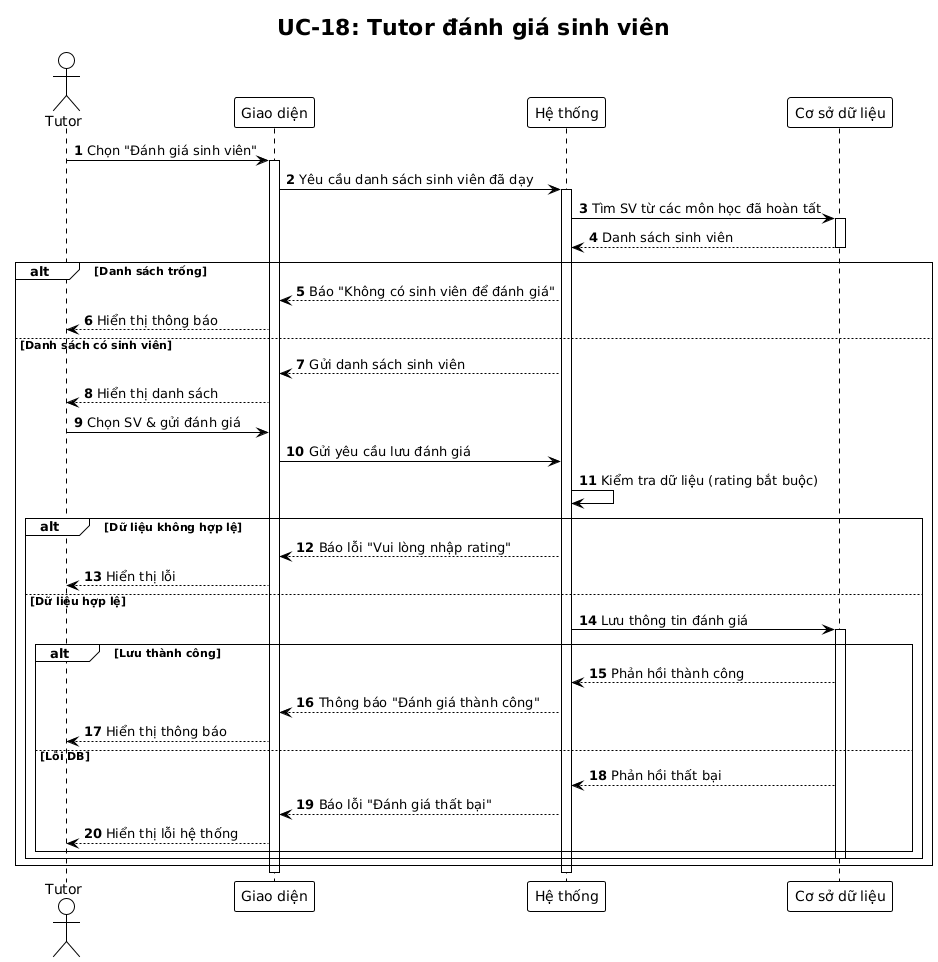
\includegraphics[scale=0.35 ]{Picture/SEUC18.png}
    \caption{Sơ đồ tuần tự Use Case 18: Tutor đánh giá sinh viên}
    \end{figure}
\end{itemize}
%========================================================================================
\subsection*{3.1.19. Use Case 19: Khoa/BM tổng hợp đánh giá}
\addcontentsline{toc}{subsection}{3.1.19. Use Case 19: Khoa/BM tổng hợp đánh giá}
\begin{itemize}
    \item Sơ đồ hoạt động
    \begin{figure}[H]
    \centering
    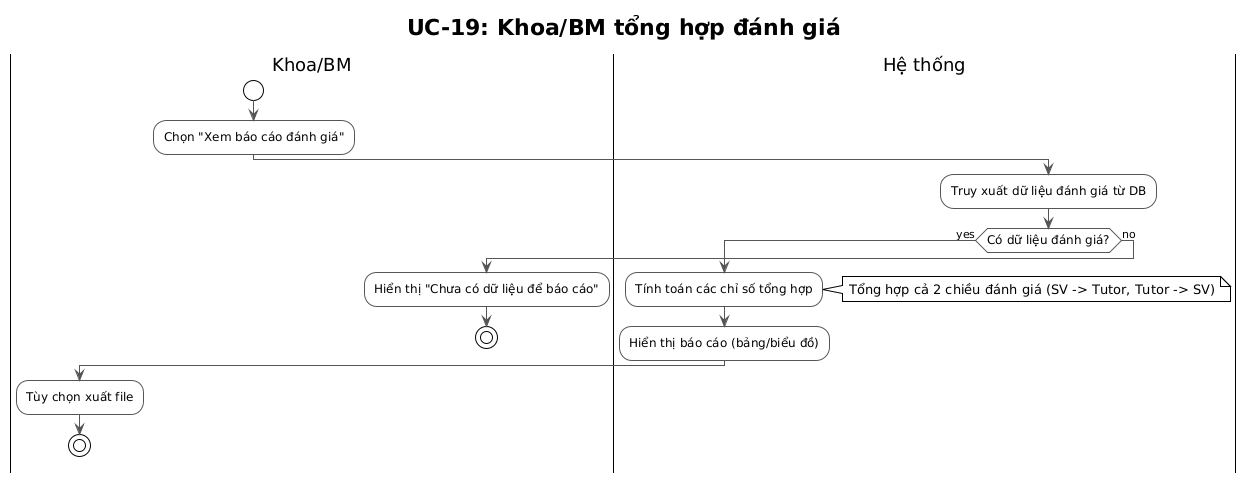
\includegraphics[scale=0.35 ]{Picture/ACUC19.png}
    \caption{Sơ đồ hoạt động Use Case 19: Khoa/BM tổng hợp đánh giá}
    \end{figure}
    \item Sơ đồ tuần tự
    \begin{figure}[H]
    \centering
    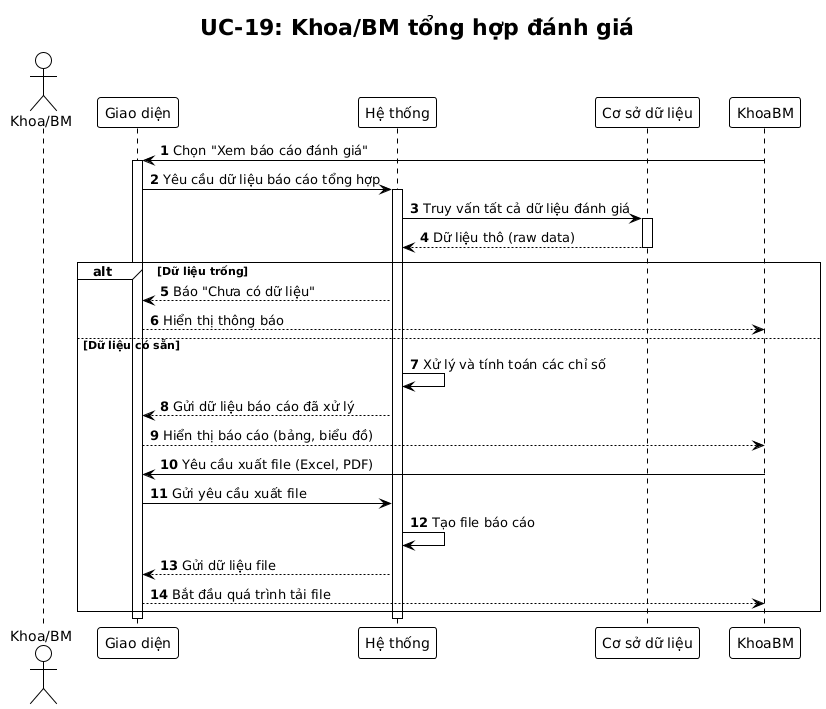
\includegraphics[scale=0.45 ]{Picture/SEUC19.png}
    \caption{Sơ đồ tuần tự Use Case 19: Khoa/BM tổng hợp đánh giá}
    \end{figure}
\end{itemize}
%========================================================================================
\subsection*{3.1.20. Use Case 20: Báo cáo kết quả học tập SV}
\addcontentsline{toc}{subsection}{3.1.20. Use Case 20: Báo cáo kết quả học tập SV}
\begin{itemize}
    \item Sơ đồ hoạt động
    \begin{figure}[H]
    \centering
    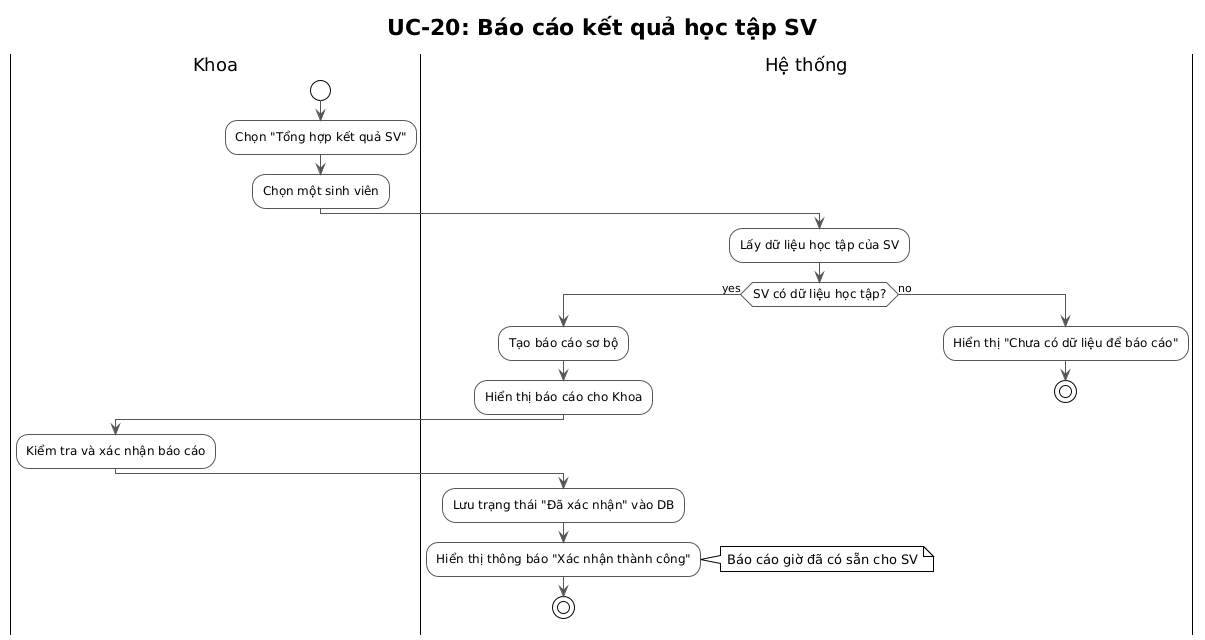
\includegraphics[scale=0.35 ]{Picture/ACUC20.png}
    \caption{Sơ đồ hoạt động Use Case 20: Báo cáo kết quả học tập SV}
    \end{figure}
    \item Sơ đồ tuần tự
    \begin{figure}[H]
    \centering
    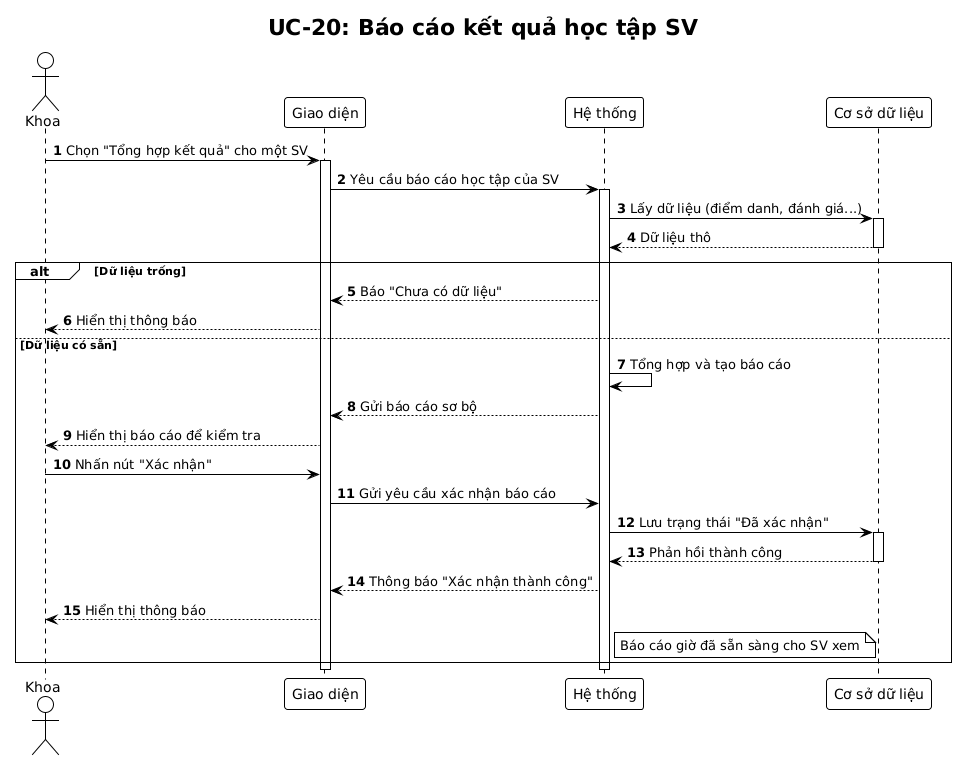
\includegraphics[scale=0.4 ]{Picture/SEUC20.png}
    \caption{Sơ đồ tuần tự Use Case 20: Báo cáo kết quả học tập SV}
    \end{figure}
\end{itemize}
%========================================================================================
\subsection*{3.1.21. Use Case 21: Báo cáo chất lượng Tutor}
\addcontentsline{toc}{subsection}{3.1.21. Use Case 21: Báo cáo chất lượng Tutor}
\begin{itemize}
    \item Sơ đồ hoạt động
    \begin{figure}[H]
    \centering
    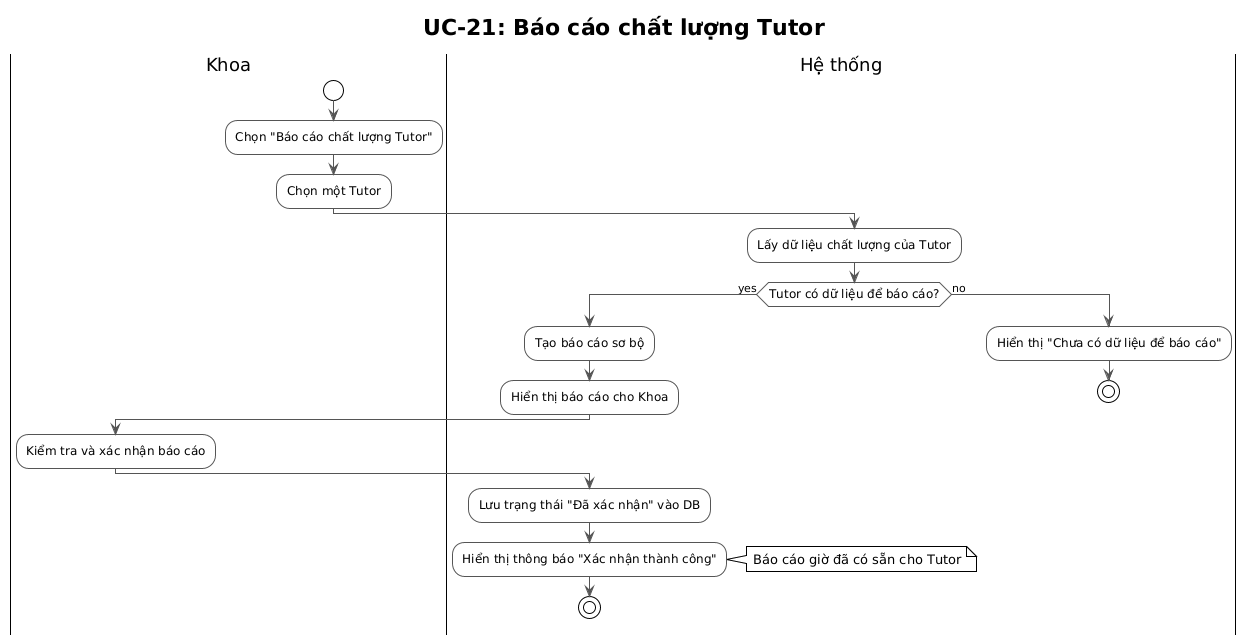
\includegraphics[scale=0.35 ]{Picture/ACUC21.png}
    \caption{Sơ đồ hoạt động Use Case 21: Báo cáo chất lượng Tutor}
    \end{figure}
    \item Sơ đồ tuần tự
    \begin{figure}[H]
    \centering
    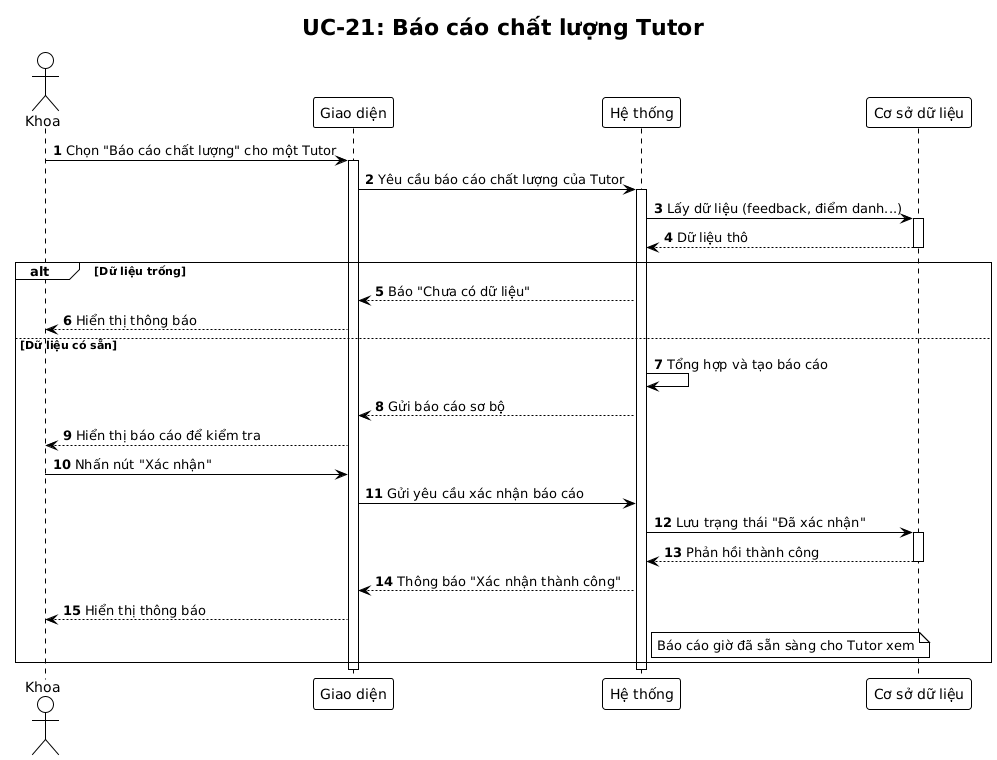
\includegraphics[scale=0.4 ]{Picture/SEUC21.png}
    \caption{Sơ đồ tuần tự Use Case 21: Báo cáo chất lượng Tutor}
    \end{figure}
\end{itemize}
%========================================================================================
\subsection*{3.1.22. Use Case 22: Báo cáo tổng hợp (Khoa, PCTSV, PĐT)}
\addcontentsline{toc}{subsection}{3.1.22. Use Case 22: Báo cáo tổng hợp (Khoa, PCTSV, PĐT)}
\begin{itemize}
    \item Sơ đồ hoạt động
    \begin{figure}[H]
    \centering
    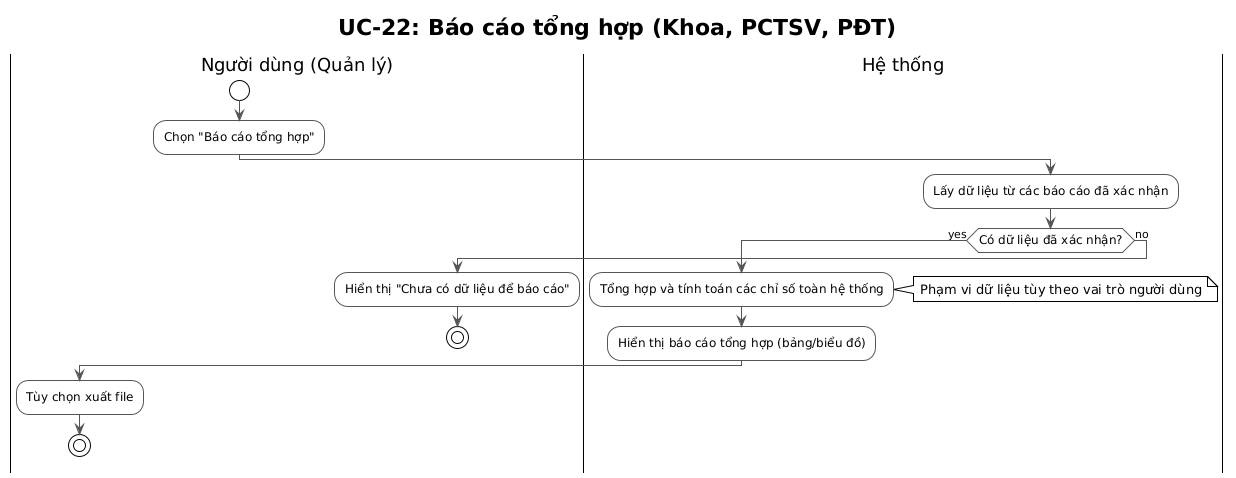
\includegraphics[scale=0.35 ]{Picture/ACUC22.png}
    \caption{Sơ đồ hoạt động Use Case 22: Báo cáo tổng hợp (Khoa, PCTSV, PĐT)}
    \end{figure}
    \item Sơ đồ tuần tự
    \begin{figure}[H]
    \centering
    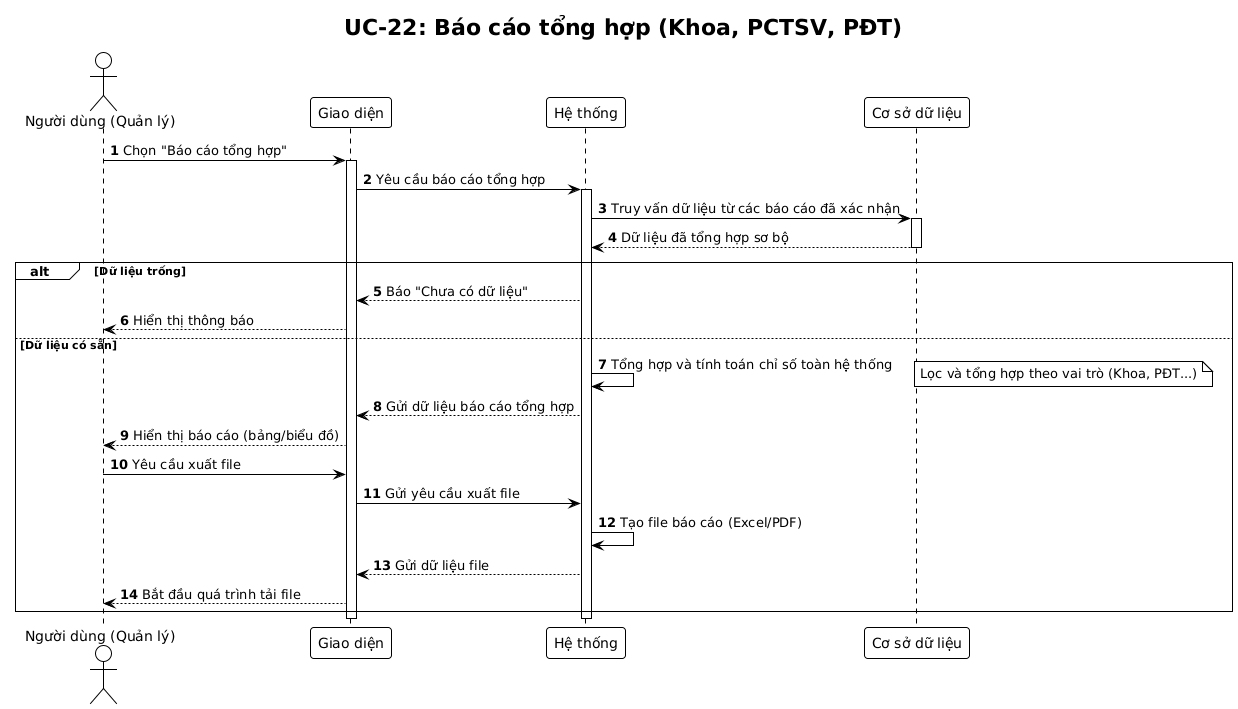
\includegraphics[scale=0.35 ]{Picture/SEUC22.png}
    \caption{Sơ đồ tuần tự Use Case 22: Báo cáo tổng hợp (Khoa, PCTSV, PĐT)}
    \end{figure}
\end{itemize}
%========================================================================================
\subsection*{3.1.23. Use Case 23: Tutor tạo chương trình học}
\addcontentsline{toc}{subsection}{3.1.23. Use Case 23: Tutor tạo chương trình học}
\begin{itemize}
    \item Sơ đồ hoạt động
    \begin{figure}[H]
    \centering
    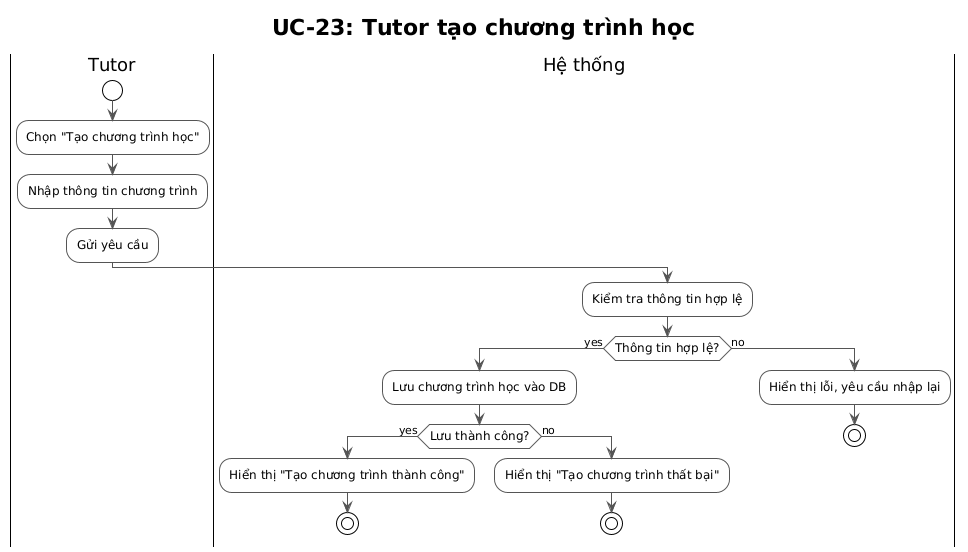
\includegraphics[scale=0.4 ]{Picture/ACUC23.png}
    \caption{Sơ đồ hoạt động Use Case 23: Tutor tạo chương trình học}
    \end{figure}
    \item Sơ đồ tuần tự
    \begin{figure}[H]
    \centering
    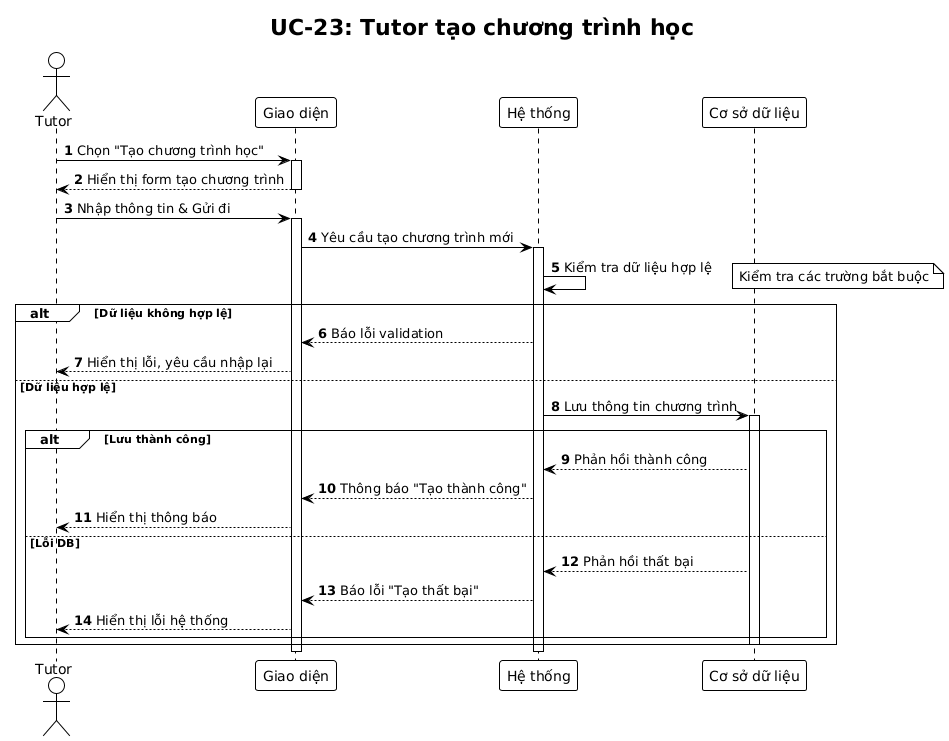
\includegraphics[scale=0.4 ]{Picture/SEUC23.png}
    \caption{Sơ đồ tuần tự Use Case 23: Tutor tạo chương trình học}
    \end{figure}
\end{itemize}
%========================================================================================
\subsection*{3.1.24. Use Case 24: SV đăng ký chương trình học thuật}
\addcontentsline{toc}{subsection}{3.1.24. Use Case 24: SV đăng ký chương trình học thuật}
\begin{itemize}
    \item Sơ đồ hoạt động
    \begin{figure}[H]
    \centering
    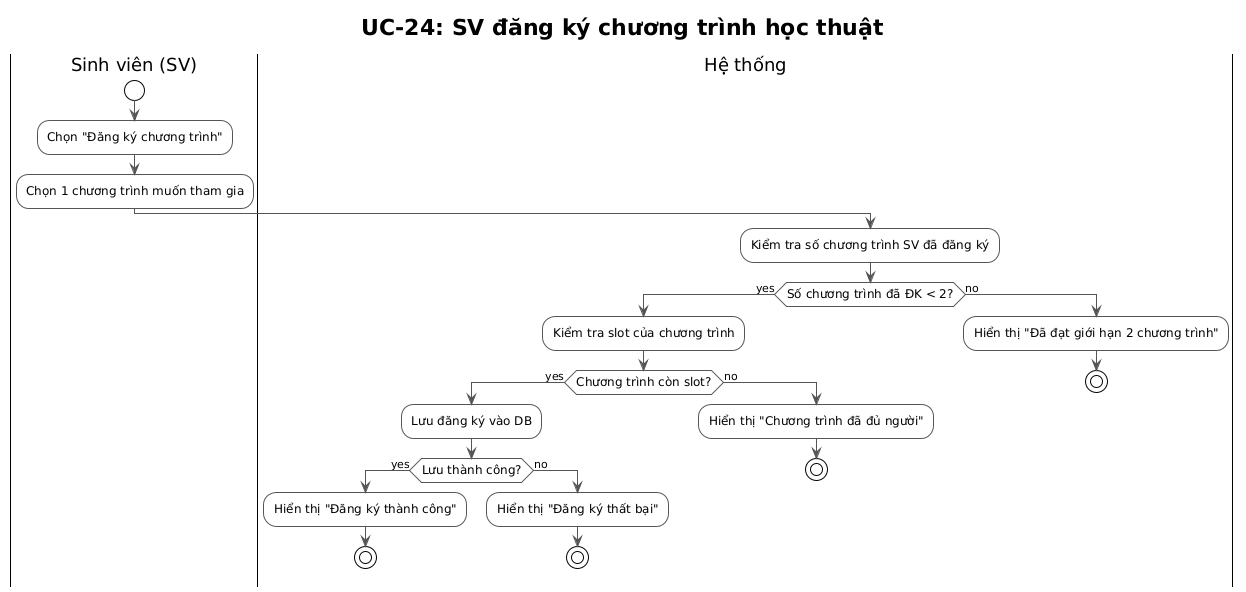
\includegraphics[scale=0.35 ]{Picture/ACUC24.png}
    \caption{Sơ đồ hoạt động Use Case 24: SV đăng ký chương trình học thuật}
    \end{figure}
    \item Sơ đồ tuần tự
    \begin{figure}[H]
    \centering
    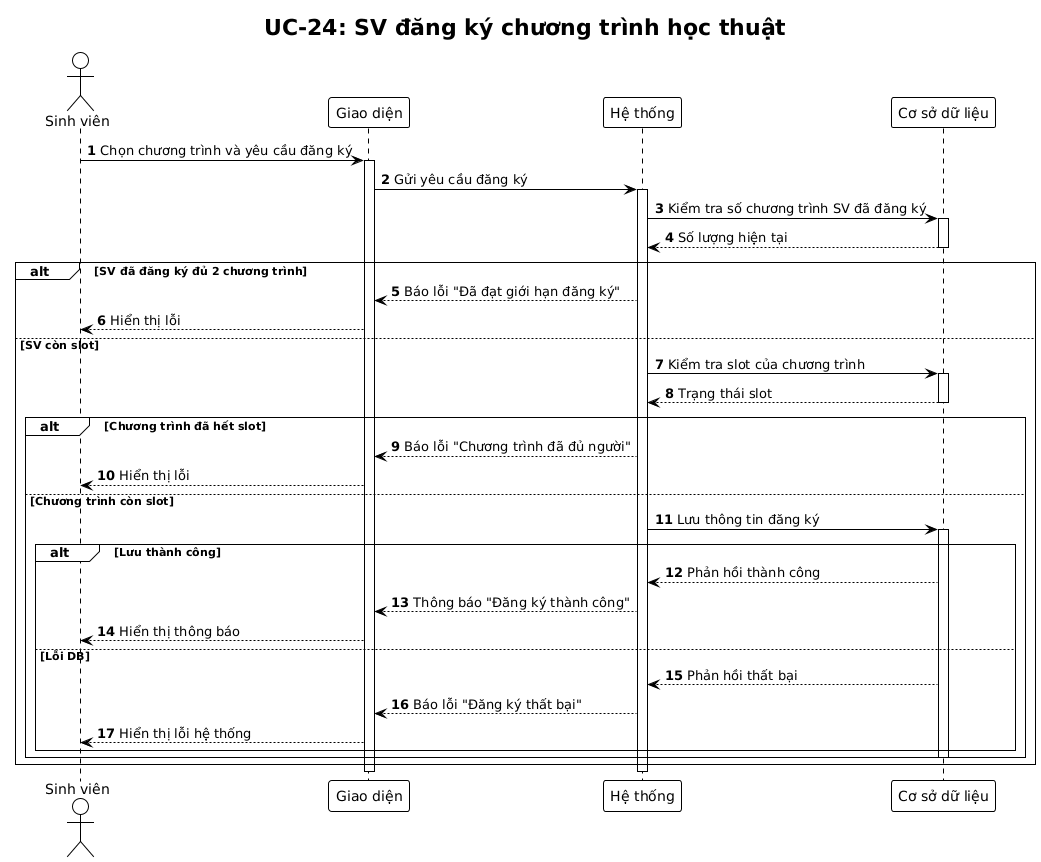
\includegraphics[scale=0.35 ]{Picture/SEUC24.png}
    \caption{Sơ đồ tuần tự Use Case 24: SV đăng ký chương trình học thuật}
    \end{figure}
\end{itemize}
%========================================================================================
\subsection*{3.1.25. Use Case 25: SV đăng ký chương trình phi học thuật}
\addcontentsline{toc}{subsection}{3.1.25. Use Case 25: SV đăng ký chương trình phi học thuật}
\begin{itemize}
    \item Sơ đồ hoạt động
    \begin{figure}[H]
    \centering
    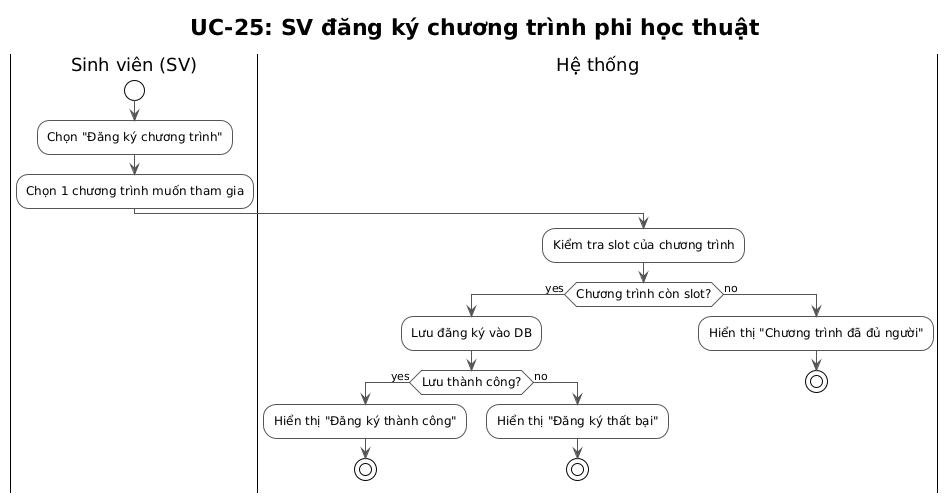
\includegraphics[scale=0.4 ]{Picture/ACUC25.png}
    \caption{Sơ đồ hoạt động Use Case 25: SV đăng ký chương trình phi học thuật}
    \end{figure}
    \item Sơ đồ tuần tự
    \begin{figure}[H]
    \centering
    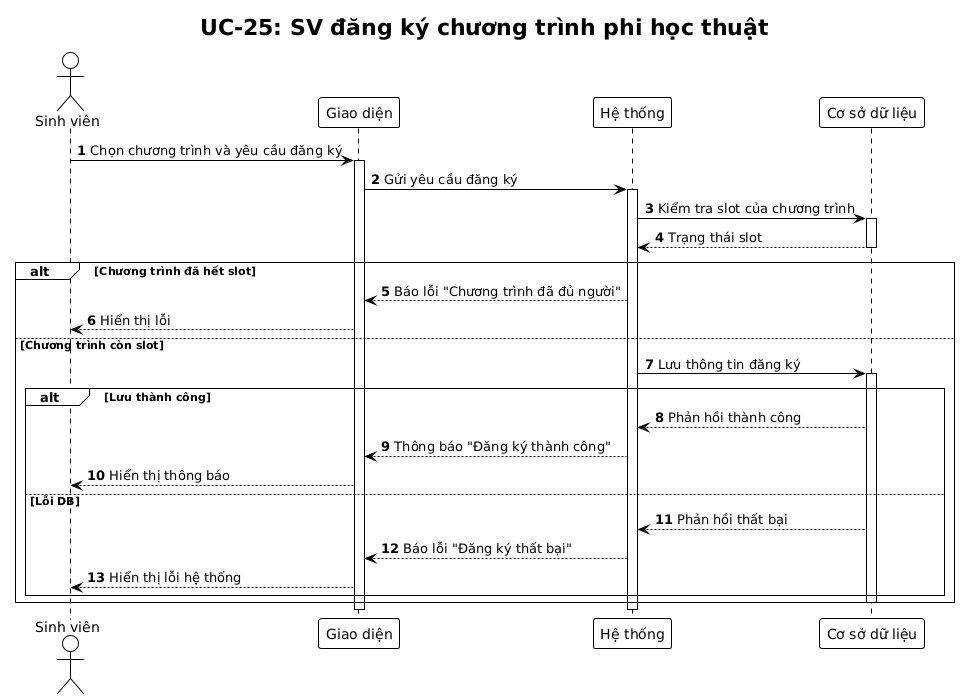
\includegraphics[scale=0.4 ]{Picture/SEUC25.png}
    \caption{Sơ đồ tuần tự Use Case 25: SV đăng ký chương trình phi học thuật}
    \end{figure}
\end{itemize}
%========================================================================================
\newpage
\section*{3.2. Giao diện}
\addcontentsline{toc}{section}{3.2. Giao diện}
Các giao diện được nhóm thiết kế trên website Figma.com. Đường dẫn: \href{https://www.figma.com/design/JVJlph8kWxybLC45mcYPDN/BTL-CNPM?node-id=0-1&t=kgGeKYXHL2xgpn6x-1}{MentorLinkUI}
\subsection*{3.2.1. Đăng ký và đăng nhập}
\addcontentsline{toc}{subsection}{3.2.1. Đăng ký và đăng nhập} 
\begin{figure}[H]
    \centering
    \setlength{\fboxsep}{2pt}      % khoảng cách giữa viền và ảnh
    \setlength{\fboxrule}{0.5pt}   % độ dày viền
    \fbox{\includegraphics[scale=0.24 ]{Picture/UI/SignUp.png}}
    \caption{Giao diện đăng ký tài khoản}
\end{figure}
\begin{figure}[H]
    \centering
    \setlength{\fboxsep}{2pt}      
    \setlength{\fboxrule}{0.5pt}   
    \fbox{\includegraphics[scale=0.24 ]{Picture/UI/SignIn.png}}
    \caption{Giao diện đăng nhập tài khoản}
\end{figure}

%========================================================================================
\newpage
\subsection*{3.2.2. Giao diện dành cho sinh viên}
\addcontentsline{toc}{subsection}{3.2.2. Giao diện dành cho sinh viên}
\subsubsection*{Trang chủ}
\begin{figure}[H]
    \centering
    \setlength{\fboxsep}{2pt}     
    \setlength{\fboxrule}{0.5pt}   
    \fbox{\includegraphics[scale=0.24]{Picture/UI/HomePage_Student.png}}
    \caption{Giao diện trang chủ của sinh viên}
\end{figure}

\subsubsection*{Đăng ký môn học}
\begin{itemize}
    \item Sinh viên chọn chức năng đăng kí môn học từ trang chủ (Hình 54), giao diện hiện ra khác môn học khả dụng và và các môn học đã đăng ký.
    \begin{figure}[H]
    \centering
    \setlength{\fboxsep}{2pt}     
    \setlength{\fboxrule}{0.5pt}   
    \fbox{\includegraphics[scale=0.24]{Picture/UI/Student_CourseRegistration.png}}
    \caption{Giao diện đăng ký môn học}
    \end{figure}
    \item Sinh viên nhấn nút "Chi tiết" để mở thông tin chi tiết của môn học.
    \begin{figure}[H]
    \centering
    \setlength{\fboxsep}{2pt}     
    \setlength{\fboxrule}{0.5pt}   
    \fbox{\includegraphics[scale=0.24]{Picture/UI/Student_CourseRegistration_Detail.png}}
    \caption{Giao diện chi tiết môn học đã đăng ký}
    \end{figure}
\end{itemize}

\subsubsection*{Tìm và ghép cặp Tutor}
\begin{itemize}
    \item Sinh viên chọn chức năng tìm và ghép cặp Tutor từ trang chủ (Hình 54), sinh viên chọn nút "thủ công", chọn môn học và hệ thống sẽ hiện danh sách Tutor để sinh viên chọ thủ công Tutor.
    \begin{figure}[H]
    \centering
    \setlength{\fboxsep}{2pt}     
    \setlength{\fboxrule}{0.5pt}   
    \fbox{\includegraphics[scale=0.24]{Picture/UI/Student_FindTutor.png}}
    \caption{Giao diện tìm và ghép cặp Tutor thủ công}
    \end{figure}
    \item Sinh viên nhấn nút "Chi tiết" để hiển thị thông tin chi tiết Tutor ở chế độ thủ công.
    \begin{figure}[H]
    \centering
    \setlength{\fboxsep}{2pt}     
    \setlength{\fboxrule}{0.5pt}   
    \fbox{\includegraphics[scale=0.24]{Picture/UI/Student_ManualPairing_Detail.png}}
    \caption{Giao diện tìm và ghép cặp Tutor thủ công}
    \end{figure}
    \item Nếu sinh viên chọn tự động (Hình 57), hệ thống sẽ tự hiển thị thông tin chi tiết của Tutor.
    \begin{figure}[H]
    \centering
    \setlength{\fboxsep}{2pt}     
    \setlength{\fboxrule}{0.5pt}   
    \fbox{\includegraphics[scale=0.24]{Picture/UI/Student_AutoPairing_Detail.png}}
    \caption{Giao diện tìm và ghép cặp Tutor tự động}
    \end{figure}
\end{itemize}

\subsubsection*{Quản lý lịch}
\begin{itemize}
    \item Sinh viên chọn chức năng quản lý lịch từ trang chủ (Hình 54), hệ thống hiển thị các môn học đã đăng ký, sinh viên chọn nút "đăng ký lịch học". 
    \begin{figure}[H]
    \centering
    \setlength{\fboxsep}{2pt}     
    \setlength{\fboxrule}{0.5pt}   
    \fbox{\includegraphics[scale=0.24]{Picture/UI/Student_ScheduleMan_ChooseCourse.png}}
    \caption{Giao diện tìm và ghép cặp Tutor thủ công}
    \end{figure}
    \item Hệ thống hiển thị lịch học để sinh viên đăng ký, sinh viên chọn nút "Đăng ký" để đăng ký lịch học phù hợp.
    \begin{figure}[H]
    \centering
    \setlength{\fboxsep}{2pt}     
    \setlength{\fboxrule}{0.5pt}   
    \fbox{\includegraphics[scale=0.24]{Picture/UI/Student_ScheduleMan_SelectTime.png}}
    \caption{Giao diện tìm và ghép cặp Tutor thủ công}
    \end{figure}
    \item Lịch học sẽ hiển thị ở Tab lịch học, có thể hủy lịch học và sửa đổi lịch học.
    \begin{figure}[H]
    \centering
    \setlength{\fboxsep}{2pt}     
    \setlength{\fboxrule}{0.5pt}   
    \fbox{\includegraphics[scale=0.24]{Picture/UI/Student_ScheduleMan_Selected.png}}
    \caption{Giao diện tìm và ghép cặp Tutor thủ công}
    \end{figure}
    \item Nếu sinh viên đổi lịch học (Hình 62), hệ thống hiển thị lịch học để sinh viên chọn.
    \begin{figure}[H]
    \centering
    \setlength{\fboxsep}{2pt}     
    \setlength{\fboxrule}{0.5pt}   
    \fbox{\includegraphics[scale=0.24]{Picture/UI/Student_ScheduleMan_ChangeTime.png}}
    \caption{Giao diện tìm và ghép cặp Tutor thủ công}
    \end{figure}
    \item Nếu sinh viên hủy lịch học (Hình 62), hệ thống sẽ gửi cảnh báo, nếu chọn "Đồng ý" hệ thống sẽ loại bỏ lịch học khỏi Tab lịch học, nếu chọn "Hủy" hệ thống sẽ hoàn tác hành động.
    \begin{figure}[H]
    \centering
    \setlength{\fboxsep}{2pt}     
    \setlength{\fboxrule}{0.5pt}   
    \fbox{\includegraphics[scale=0.24]{Picture/UI/Student_ScheduleMan_DiscardTime.png}}
    \caption{Giao diện tìm và ghép cặp Tutor thủ công}
    \end{figure}
\end{itemize}
